% 设置 biblatex 额外选项
% \PassOptionsToPackage{gbpub=false, gbtype=false}{biblatex}

% 载入 SJTUThesis 模版
% \documentclass[degree=doctor, zihao=-4, language=english, review]{sjtuthesis}
\documentclass[degree=master, zihao=-4]{sjtuthesis}
% \documentclass[degree=bachelor, openany, oneside]{sjtuthesis}
% \documentclass[degree=course, language=english, openright, twoside]{sjtuthesis}
% 选项
%   degree=[doctor|master|bachelor|course],     % 必选,学位类型
%   language=[chinese|english],                 % 可选(默认:chinese),论文的主要语言
%   bibstyle=[gb7714-2015|gb7714-2015ay|ieee],  % 可选(默认:gb7714-2015),参考文献样式
%   review,                                     % 可选(默认:关闭),盲审模式

% 所有其它可能用到的包都统一放到这里了,可以根据自己的实际添加或者删除。
\usepackage{sjtuthesis}

% 定义图片文件目录与扩展名
\graphicspath{{figure/}}
\DeclareGraphicsExtensions{.pdf,.eps,.png,.jpg,.jpeg}

% 导入参考文献数据库
\addbibresource{bib/thesis.bib}

% 信息录入,必须在导言区进行!
% !TEX root = ../thesis.tex

%TC:ignore

\title{上海交通大学学位论文 \LaTeX{} 模板示例文档}
\author{某\quad{}某}
\studentid{0010900990}
\supervisor{某某教授}
% \assisupervisor{某某教授}
\degree{工学硕士}
\major{某某专业}
\department{某某系}
\coursename{某某课程}
\date{2014年12月17日}
% \fund{国家 973 项目 (No. 2025CB000000) \\ 国家自然科学基金 (No. 81120250000)}
\keywords{上海交大, 饮水思源, 爱国荣校}

\entitle{A Sample Document for \LaTeX-based SJTU Thesis Template}
\enauthor{Mo Mo}
\ensupervisor{Prof. Mou Mou}
% \enassisupervisor{Prof. Uom Uom}
\endegree{Master of Engineering}
\enmajor{A Very Important Major}
\endepartment{Depart of XXX}
\endate{Dec. 17th, 2014}
% \enfund{National Basic Research Program of China (Grant No. 2025CB000000) \\
%   National Natural Science Foundation of China (Grant No. 81120250000)}
\enkeywords{SJTU, master thesis, XeTeX/LaTeX template}

%TC:endignore


% 自定义项目标签名称
% \sjtuSetLabel{
%   listfigure = {图\quad 录},
%   listtable  = {表\quad 录}
% }

\begin{document}

% 无编号内容:中英文论文封面、授权页
\maketitle
\makeDeclareOriginality[pdf/originality.pdf]
\makeDeclareAuthorization

% 使用罗马数字对前言编号
\frontmatter

% 摘要
% !TEX root = ../thesis.tex

\begin{abstract}
  横洋科技股份有限公司是由上海交通大学博士团队创立的一家海上智能系统研发企业,
  致力于运用人工智能和大数据技术重构海上无人系统,服务军民两用,
  为实现国家海洋强国梦贡献智慧力量,为打造“中国智造”的世界名片谱写辉煌。


  摘要页的下方注明本文的关键词(4~6个)。
\end{abstract}

\begin{enabstract}
  Shanghai Jiao Tong University (SJTU) is a key university in China. SJTU was
  founded in 1896. It is one of the oldest universities in China. The University
  has nurtured large numbers of outstanding figures include JIANG Zemin, DING
  Guangen, QIAN Xuesen, Wu Wenjun, WANG An, etc.

  SJTU has beautiful campuses, Bao Zhaolong Library, Various laboratories. It
  has been actively involved in international academic exchange programs. It is
  the center of CERNet in east China region, through computer networks, SJTU has
  faster and closer connection with the world.
\end{enabstract}


% 目录、插图目录、表格目录
\tableofcontents
\listoffigures
\listoftables
\listofalgorithms

% 主要符号、缩略词对照表
% !TEX root = ../thesis.tex

%TC:ignore

\begin{nomenclature}{rl}
\label{chap:symb}
  $\epsilon$     & 介电常数 \\  
  $\mu$ 		& 磁导率 \\
  $\epsilon$     & 介电常数 \\
  $\mu$ 		& 磁导率 \\
  $\epsilon$     & 介电常数 \\
  $\mu$ 		& 磁导率 \\
  $\epsilon$ 	& 介电常数 \\
  $\mu$ 		& 磁导率 \\
  $\epsilon$     & 介电常数 \\
  $\mu$ 		& 磁导率 \\
  $\epsilon$     & 介电常数 \\
  $\mu$ 		& 磁导率 \\
  $\epsilon$     & 介电常数 \\
  $\mu$ 		& 磁导率 \\
  $\epsilon$ 	& 介电常数 \\
  $\mu$ 		& 磁导率 \\
  $\epsilon$     & 介电常数 \\
  $\mu$ 		& 磁导率 \\
  $\epsilon$     & 介电常数 \\
  $\mu$ 		& 磁导率 \\
  $\epsilon$     & 介电常数 \\
  $\mu$ 		& 磁导率 \\
  $\epsilon$ 	& 介电常数 \\
  $\mu$ 		& 磁导率 \\
  $\epsilon$     & 介电常数 \\
  $\mu$ 		& 磁导率 \\
  $\epsilon$     & 介电常数 \\
  $\mu$ 		& 磁导率 \\
  $\epsilon$     & 介电常数 \\
  $\mu$ 		& 磁导率 \\
  $\epsilon$ 	& 介电常数 \\
  $\mu$ 		& 磁导率 \\
  $\epsilon$     & 介电常数 \\
  $\mu$ 		& 磁导率 \\
  $\epsilon$     & 介电常数 \\
  $\mu$ 		& 磁导率 \\
  $\epsilon$     & 介电常数 \\
  $\mu$ 		& 磁导率 \\
  $\epsilon$ 	& 介电常数 \\
  $\mu$ 		& 磁导率 \\
  $\epsilon$     & 介电常数 \\
  $\mu$ 		& 磁导率 \\
  $\epsilon$     & 介电常数 \\
  $\mu$ 		& 磁导率 \\
  $\epsilon$     & 介电常数 \\
  $\mu$ 		& 磁导率 \\
  $\epsilon$ 	& 介电常数 \\
  $\mu$ 		& 磁导率 \\
  $\epsilon$     & 介电常数 \\
  $\mu$ 		& 磁导率 \\
  $\epsilon$     & 介电常数 \\
  $\mu$ 		& 磁导率 \\
  $\epsilon$     & 介电常数 \\
  $\mu$ 		& 磁导率 \\
\end{nomenclature}

%TC:endignore


% 使用阿拉伯数字对正文编号
\mainmatter

% 正文内容

%# -*- coding: utf-8-unix -*-
% !TEX program = xelatex
% !TEX root = ../thesis.tex
% !TEX encoding = UTF-8 Unicode
%%==================================================
%% chapter01.tex for SJTU Master Thesis
%%==================================================

%\bibliographystyle{sjtu2}%[此处用于每章都生产参考文献]

\newcommand{\bodyframe}{\left\{ \mathbf{b} \right\}}
\newcommand{\NEDframe}{\left\{ \mathbf{n} \right\} }

\chapter{船体运动模型}
\label{chap:chapter01}

本章介绍船体运动模型,主要分为单自由首要控制模型、3自由度操纵性模型、3自由度动力定位模型、
4自由度带有横摇补偿的操纵性模型。

\section{坐标系}
\subsection{北东地坐标系}
北东地(North-East-Down: NED)坐标系$\NEDframe=(x_n, y_n, z_n)$是
常用的导航坐标系,通常定义在地球表面的切平面上,其中$x$轴指向地球北,$y$轴指向地球东,
$z$轴垂直于地球表面并指向下。通常对于海上船舶,经纬度的变化并不大,我们可以假定$\NEDframe$
是惯性参考系。

北东地坐标系在程序里也称Marine coordinate,与之对应的是UTM坐标系
(UTM-x指向正东,UTM-y指向正北)。

\subsection{笛卡尔坐标系}
笛卡尔(Cartesian)坐标系如图\ref{fig:3Dcartesian}在数学中是一种正交坐标系,
由法国数学家勒内·笛卡尔引入而有此名。二维的直角坐标系是由两条相互垂直、
相交于原点的数线构成的。在平面内,任何一点的坐标是根据数轴上对应的点的坐标设定的。
在平面内,任何一点与坐标的对应关系,类似于数轴上点与坐标的对应关系。

\subsection{随体坐标系}
随体坐标系 $\bodyframe$ 始终跟随船体的运动,通常我们随体坐标系的原点$o_b$置于船体中轴线上,
并位于船尾甲板处(船体上比较容易接触到某一点)。
一般我们用六个变量来描述船体的运动,主要分为平动($x,y,z$)和转动($\phi, \theta, \psi$),
具体的描述和符号见图\ref{fig:Coordinate}和表\ref{tab:notation}。图中,CoG在随体坐标系
中相对于$o_b$的坐标可表示为$\mathbf{r}_g = (x_g,y_g, z_g)^T$

\begin{figure}[!htp]
  \centering
  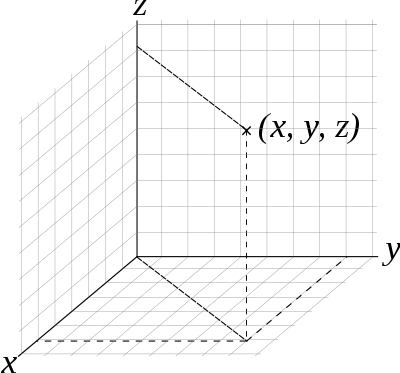
\includegraphics[width=9cm]{chapter01/3D_Cartesian.png}
  \bicaption[笛卡尔坐标系]
    {笛卡尔坐标系}
    {Cartesian coordinate system}
  \label{fig:3Dcartesian}
\end{figure}

\begin{figure}[!htp]
  \centering
  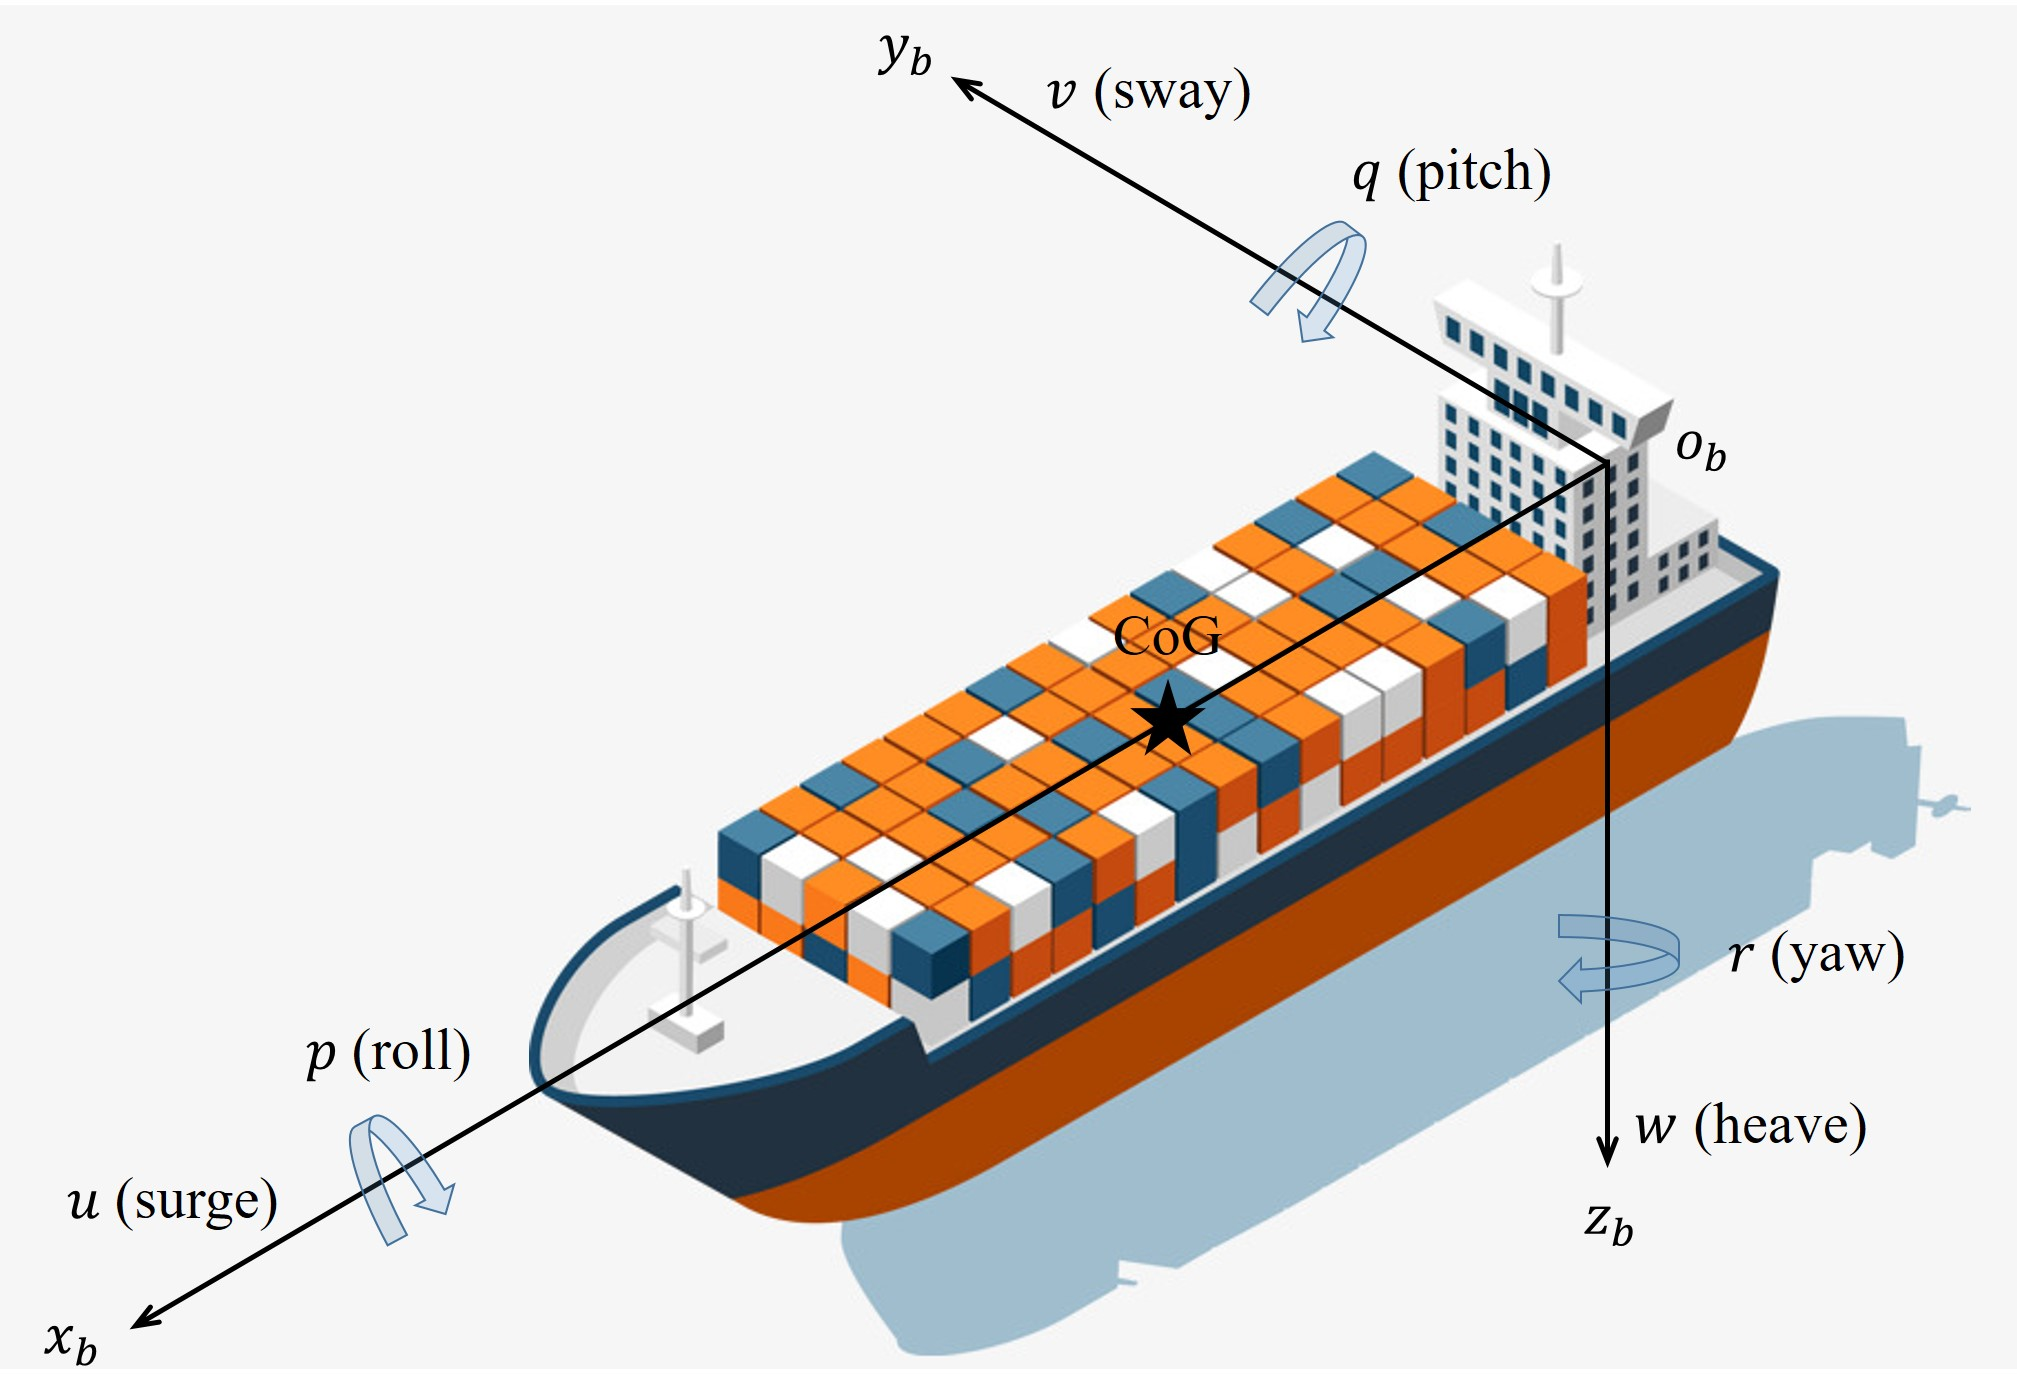
\includegraphics[width=13cm]{chapter01/Coordinate.jpg}
  \bicaption[在随体坐标系中,船体六自由度的速度 $u,v,w,p,q,r$]
    {在随体坐标系 $\bodyframe$ 中,船体六自由度的速度 $u,v,w,p,q,r$}
    {The 6DoF velocities $u,v,w,p,q,r$ in the body-fixed reference frame
    $\bodyframe=(x_b, y_b, z_b)$  }
  \label{fig:Coordinate}
\end{figure}


% Table generated by Excel2LaTeX from sheet 'Sheet1'
\begin{table}[htbp]
  \centering
  \caption{描述船体运动的常用符号}
    \begin{tabular}{llll}
    \toprule
    自由度(DOF) & 力/力矩  & 线/角速度 & 位置/欧拉角 \\
    \midrule
    1 \quad surge & $X$     & $u$     & $x$ \\
    2 \quad sway &  $Y$     & $v$     & $y$ \\
    3 \quad heave & $Z$     & $w$     & $z$ \\
    4 \quad roll & $K$     &  $p$     & $\phi$ \\
    5 \quad pitch & $M$     & $q$     & $\theta$ \\
    6 \quad yaw & $N$     &   $r$     & $\psi$ \\
    \bottomrule
    \end{tabular}%
  \label{tab:notation}%
\end{table}%

\subsection{运动方程}


\section{海洋环境载荷}
风、浪、流


\section{三自由度操纵性方程}
三自由度操纵性方程只考虑低频的surge, sway和yaw方向上的运动,并假定船体以恒定的速度前行
$u=U$,忽略海流的作用,

\begin{equation}
  \label{eq:3dofmaneuvering}
  (\bm{M}_{RB}+\bm{M}_A) \dot{\bm{v}}+(\bm{C}_{RB}(\bm{v})+
  \bm{C}_{A}(\bm{v})+\bm{D})\bm{v}=\bm{\tau}+\bm{\tau}_{wind}+
  \bm{\tau}_{wave}
\end{equation}

\begin{equation}
  \label{eq:3doftransform}
  \dot{\bm{\eta}}=\bm{J}(\bm{\eta})\bm{v}=
  \begin{bmatrix}
    \cos{\psi} & -\sin{\psi} & 0 \\
    \sin{\psi} & \cos{\psi} & 0 \\
    0 & 0 & 1
  \end{bmatrix}
  \bm{v}
\end{equation}

其中,$\bm{v}=(u,v,r)^T$是随体坐标系$\bodyframe$下的速度,$\bm{\eta}=(N,E,\psi)^T$
是北东地坐标系$\NEDframe$下的位置, $\bm{\tau},\bm{\tau}_{wind}, \bm{\tau}_{wave}$
分别为作用在船体上的控制力、风力和流力,均相对于随体坐标系。

\begin{equation}
  \label{eq:massmatrix}
  \bm{M}_{RB}=\begin{pmatrix}
            m & 0 & 0 \\
            0 & m & mx_g \\
            0 & mx_g & I_z
          \end{pmatrix},
  \quad
  \bm{M}_{A}=\begin{pmatrix}
            -X_{\dot{u}} & 0 & 0 \\
            0 & -Y_{\dot{v}} & -Y_{\dot{r}} \\
            0 & -Y_{\dot{r}} & -N_{\dot{r}}
          \end{pmatrix}
\end{equation}
相对于随体坐标系原点$o_b$的附加质量$\bm{M}_{A}$可以通过势流计算软件得到;
{\color{red} 在无人船程序中,我们采用原点位于重心的随体坐标系
$\left\{ \bm{b}_{CoG} \right\}$,可使得质量矩阵为对角矩阵。同时推力、定位系统获得的位置、规控模块均相对于
$\left\{ \bm{b}_{CoG} \right\}$}。
势流阻尼$\bm{C}_{A}(\bm{v})$可通过势流计算软件得到,有时可以忽略,
\begin{equation}
  \label{eq:potentialdampingmatrix}
  \bm{C}_{A}(\bm{v})=
          \begin{pmatrix}
            0 & 0 &  Y_{\dot{v}}v+Y_{\dot{r}}r \\
            0 & 0 & -X_{\dot{u}}u \\
            -Y_{\dot{v}}v-Y_{\dot{r}}r & X_{\dot{u}}u & 0
          \end{pmatrix}
\end{equation}

\begin{equation}
  \label{eq:coupleddampingmatrix}
  \bm{C}_{RB}(\bm{v})=
         \begin{pmatrix}
            0 & 0 & -m(x_g r +v) \\
            0 & 0 & mu \\
            m(x_g r +v) & -mu & 0
          \end{pmatrix}
\end{equation}

线性阻尼矩阵$\bm{D}$可用模型试验辨识或者经验公式得到。线性阻尼通常在船舶低速航行的时候
占主导,而高速的时候,非线性阻尼也需要考虑,参见\cite{fossen2011handbook}第136页。
\begin{equation}
  \label{eq:lineardampingmatrix}
  \bm{D}=\begin{pmatrix}
            -X_{u} & 0 & 0 \\
            0 & -Y_{v} & -Y_r \\
            0 & -N_v & -N_r
          \end{pmatrix}
\end{equation}


\section{三自由度动力定位方程}
动力定位系统假定船体的航速很小,通常只考虑线性阻尼项,
\begin{equation}
  \label{eq:3dofdp}
  (\bm{M}_{RB}+\bm{M}_A) \dot{\bm{v}}+\bm{D}\bm{v}=\bm{\tau}+\bm{\tau}_{wind}+
  \bm{\tau}_{wave}+\bm{\tau}_{current}
\end{equation}

\begin{equation}
  \label{eq:3doftransformdp}
  \dot{\bm{\eta}}=\bm{J}(\bm{\eta})\bm{v}
\end{equation}
其中,$\bm{M}_{RB},\bm{M}_A, \bm{D}, \bm{J}(\bm{\eta})$和3DoF操纵性方程是一样的,通常我们假定风力和流力是缓变的,并根据经验公式估算得到。
\section{单自由度首向控制方程}




\section{四自由度横摇补偿操纵性方程}


\section{参数辨识}

假定一个弹簧振子的质量为$m$, 弹簧刚度为$k$,则
\begin{equation}
  \begin{aligned}
    &F=k \Delta x \\
    &T= 2 \pi \sqrt{\frac{m}{k}}
  \end{aligned}
\end{equation}

进而假设船体的质量为$m$,其转动惯量为$I$, 则船体受的恢复力矩为
\begin{equation}
  \begin{aligned}
    \frac{mg}{2} \tan(\alpha)   &\approx   \frac{mg}{2} \alpha \\
    &=\frac{mg}{2}\frac{\Delta \theta d}{L}
  \end{aligned}
\end{equation}
\begin{equation}
  M=\frac{mgd^2 }{L} \Delta \theta
\end{equation}
运用单摆原理,可得周期为
\begin{equation}
  T=2 \pi \sqrt{\frac{I}{\frac{mgd^2 }{L} }} = 2 \pi \sqrt{\frac{I L}{mgd^2}}
\end{equation}


\begin{figure}[!htp]
  \centering
  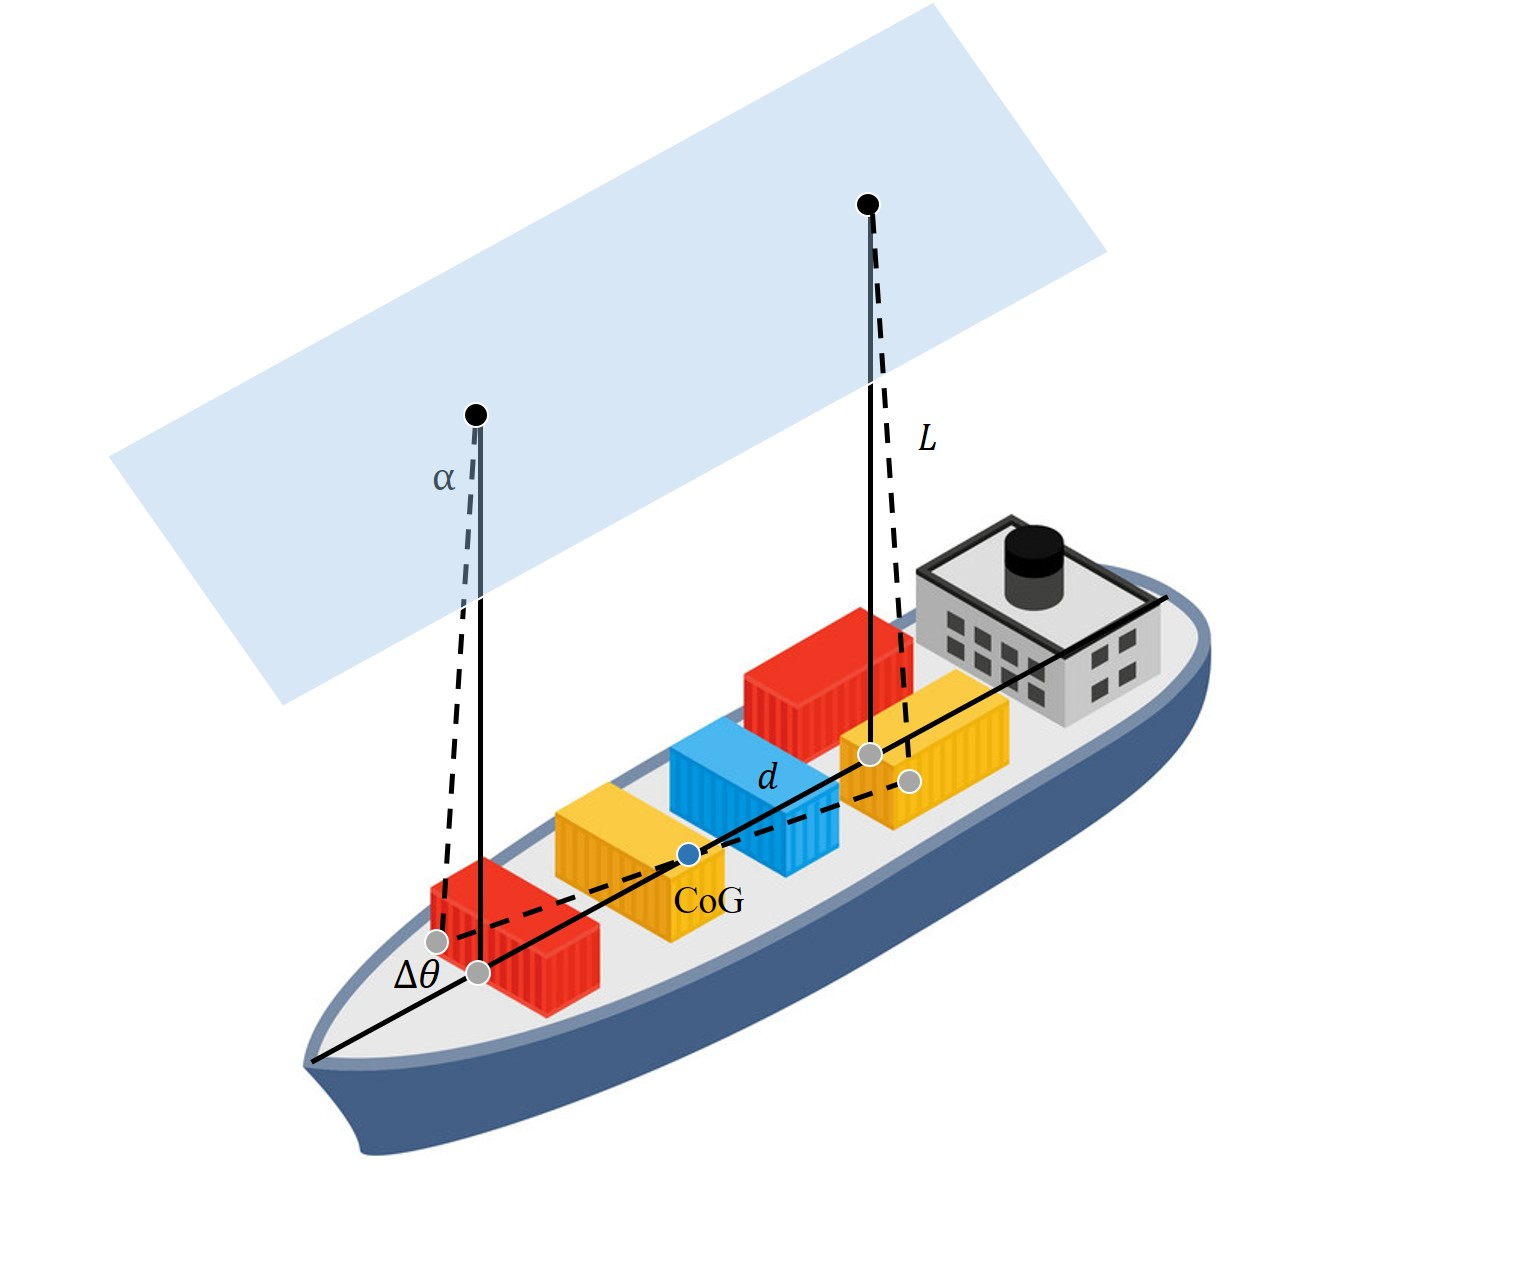
\includegraphics[width=14cm]{chapter01/InertialMeasurement.jpg}
  \bicaption[转动惯量的测量原理]
    {转动惯量的测量原理}
    {Sketch of Inertial Measurement}
  \label{fig:InertialMeasurement}
\end{figure}


\subsection{质量}
重心坐标一般相对于$o_b$

%# -*- coding: utf-8-unix -*-
% !TEX program = xelatex
% !TEX root = ../thesis.tex
% !TEX encoding = UTF-8 Unicode
%%==================================================
%% chapter01.tex for SJTU Master Thesis
%%==================================================

%\bibliographystyle{sjtu2}%[此处用于每章都生产参考文献]


\chapter{控制器}
\label{chap:chapter02}
船舶系统按不同的推进器配置可分为欠驱动(Underactuated systems)和全驱动(fully-actuated
systems)系统。通常所说的动力定位船舶或者平台即为全驱动系统,这类系统的输入量不少于控制量。
而欠驱动船舶是输入比要控制的量少的一类典型系统。
本章介绍船舶控制器,主要包括PID控制器,轨迹跟踪算法和推力分配算法。

\section{推力分配}
\subsection{推进器简介}
船用推进器主要包括隧道式螺旋桨、全回转螺旋桨、固定式螺旋桨加舵以及泵推。其简图如\ref{fig:thrustertype}

\begin{figure}[!htp]
  \centering
  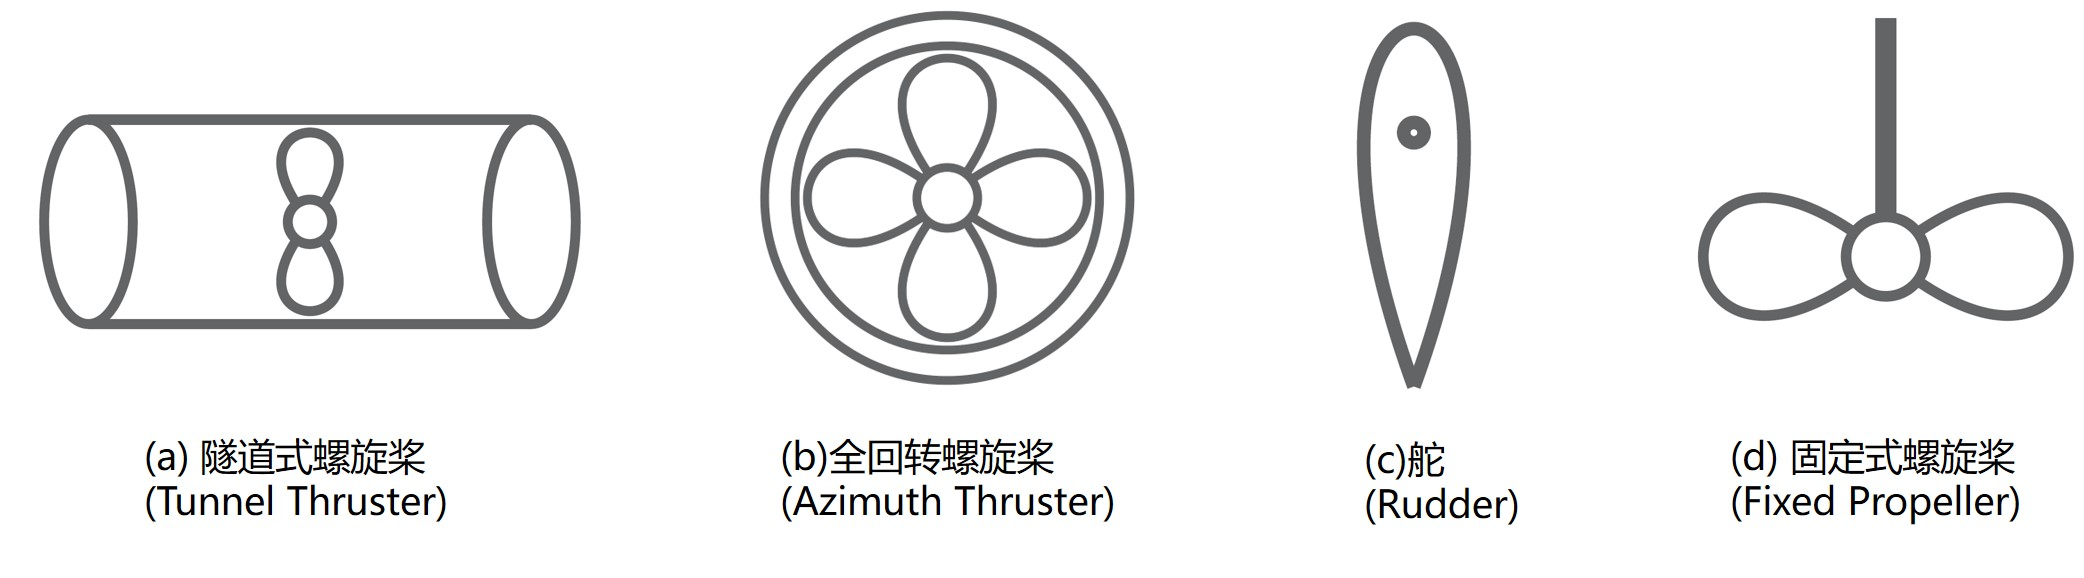
\includegraphics[width=15cm]{chapter02/thrustertype.jpg}
  \bicaption[常见船舶推进器示意图]
    {常见船舶推进器示意图}
    {Sketch of common thrusters of vessel}
  \label{fig:thrustertype}
\end{figure}

对于每种推进器,其推力可根据船级社DNVGL的规范 \cite{DNVGL2016DP}估算得到。
\begin{equation}
  \label{eq:effectivethrust}
    {\tau}_{e} = \beta_T {\tau}_{n}
\end{equation}
其中,${\tau}_{e}$称为有效推力,${\tau}_{n}$是名义推力,$\beta_T$是
推力损失系数。
\begin{equation}
  \label{eq:nominalthrust}
    {\tau}_{n} = \eta_1 \eta_2 \left(D\times P\right)^{\frac{2}{3}}
\end{equation}
其中,$D$是以米(m)为单位的螺旋桨直径,$P$是以千瓦(kW)为单位的推进器功率。$\eta_1$和
$\eta_2$的取值参见DNVGL的规范。

对于舵,其推力
\begin{equation}
  \begin{aligned}
  \label{eq:rudderthrust}
    {\tau}_{surge} &= {\tau}_e (1-C_x \alpha^2) \\
    {\tau}_{sway} &= {\tau}_e C_y \alpha \\
    C_x &= 0.02 C_y  \\
    C_y &= 0.0126 k_1 k_2 \frac{A_r}{D^2}
  \end{aligned}
\end{equation}
其中$\alpha$是以度$(^{\circ})$为单位的舵角,一般舵角不会超过$30^{\circ}$。
$A_r$是舵可转动部分的面积。$k_1$和$k_2$的取值参见规范。

\subsection{推力分配模型}
推力分配算法将广义力作为输入,通过建模并优化得到每个推进器上的转速和推力。

\begin{figure}[!htp]
  \centering
  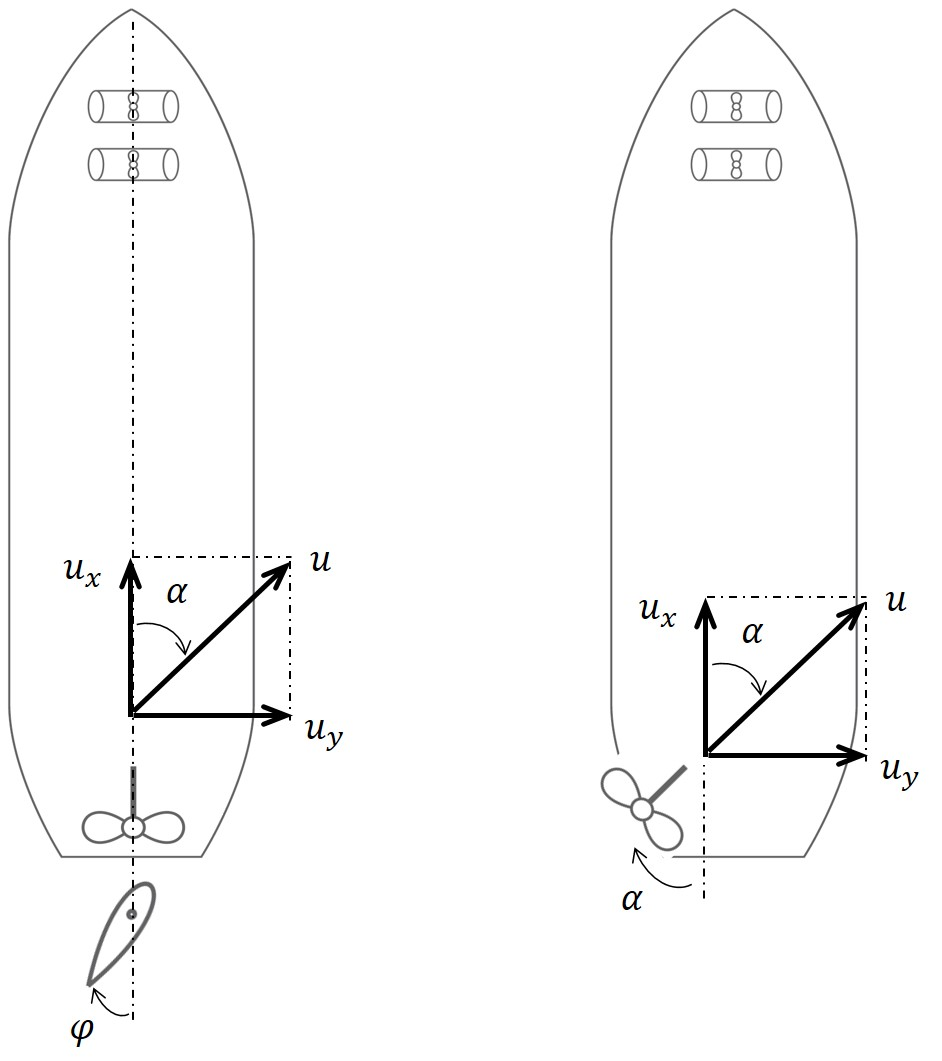
\includegraphics[width=10cm]{chapter02/thrusteralpha.jpg}
  \bicaption[螺旋桨角度的定义]
    {螺旋桨角度的定义}
    {Sketch of azimuth of each thruster}
  \label{fig:thrusteralpha}
\end{figure}


\begin{equation}
  \label{eq:eachthruster}
    {\bm{\tau}}(t) = \bm{B}(\bm{\alpha} )  \cdot \bm{u}
\end{equation}
其中,$\bm{u}=[u_1,u_2, \dots, u_m]^T \in \mathbb{R}^m$ 代表每个推进器产生的推力,
$\bm{\alpha}=[\alpha_1, \alpha_2, \dots, \alpha_m ]^T \in \mathbb{R}^m$ 代表
每个推进器的角度,其定义参见图\ref{fig:thrusteralpha}。
假设在随体坐标系中,推进器相对于重心的位置为$(l_{xi},l_{yi})$, 则矩阵
$\bm{B}(\bm{\alpha} ) \in \mathbb{R}^{3 \times m}$可得
\begin{equation}
  \label{eq:Balpha}
\bm{B}(\bm{\alpha})=\left[\begin{array}{cccc}{
\cos \alpha_{1}} & {\cos \alpha_{2}} & \cdots & {\cos \alpha_{m}} \\
{\sin \alpha_{1}} & {\sin \alpha_{2}}  & \cdots & {\sin \alpha_{m}} \\
{l_{x 1} \sin \alpha_{1}-l_{y 1} \cos \alpha_{1}} &
{l_{x 2} \sin \alpha_{2}-l_{y 2} \cos \alpha_{2}} &
\cdots  &
{l_{x m} \sin \alpha_{m}-l_{y m} \cos \alpha_{m}}\end{array}\right]
\end{equation}

我们假设推力和螺旋桨转速$n$呈二次关系
\begin{equation}
  \label{eq:thrustrotation}
    u_i= K_i n_i |n_i|
\end{equation}
其中,$K_i$可以从推力测量实验(详见\ref{sec:parameters}节)得到。

我们将推力分配问题转化为带有线性约束的二次规划问题(Quadratic Programming)
\cite{johansen2004constrained}, 目前我们采用Mosek或osqp求解器来计算优化解。
\begin{equation}
  \label{eq:qpmin}
    \begin{aligned}
      \min J(\Delta \bm{\alpha}, \Delta \bm{u}, \bm{s})
      &= \sum_{i=1}^{m} \left(
      \frac{\mathrm{d} W_{i}}{\mathrm{d} u_{i}}\left( u_{0, i} \right)
      \Delta u_{i}+
      \frac{\mathrm{d}^{2} W_{i}}{\mathrm{d} u_{i}^{2}}\left(u_{0, i}\right)
      \Delta u_{i}^{2} \right)+
      \Delta \bm{\alpha}^{T} \bm{\Omega} \Delta \bm{\alpha}+\bm{s}^{T} \bm{Q} \bm{s} \\
      &+\frac{\mathrm{d}}{\mathrm{d}\alpha}\left(\frac{\rho}{\varepsilon+
      \operatorname{det}\left(\bm{B}(\bm{\alpha})\bm{B}^{T}(\bm{\alpha})\right)}\right)
      _{\alpha=\alpha_{0}} \cdot \Delta \bm{\alpha} \\
      &=\bm{g}_{\Delta u}^{T} \cdot \Delta \bm{u}+\Delta \bm{u}^{T} \bm{Q}_{\Delta u}
      \Delta \bm{u}+\bm{s}^{T} \bm{Q} \bm{s}+\Delta \bm{\alpha}^{T}
      \bm{\Omega} \Delta \bm{\alpha}+\bm{d}_{\rho}^{T} \Delta \bm{\alpha}
    \end{aligned}
\end{equation}

\begin{equation}
  \label{eq:qpconstraints}
    \begin{aligned}
      \text{subject to } \\
      &\bm{s}+\bm{B}\left(\bm{\alpha}_{0}\right) \cdot \Delta \bm{u}+
      \frac{\partial}{\partial \bm{\alpha}}(\bm{B}(\bm{\alpha}) \bm{u})
      _{\bm{\alpha}=\bm{\alpha_{0}}} \cdot \Delta \bm{\alpha}
      =\bm{\tau}-\bm{B}\left(\bm{\alpha}_{0}\right) \cdot \bm{u}_{0} \\
      &\underline{\Delta \bm{u}} \leq \Delta \bm{u} \leq \overline{\Delta \bm{u}}
      \\ &\underline{\Delta \bm{\alpha}} \leq \Delta \bm{\alpha} \leq \overline{\Delta \bm{\alpha}}
    \end{aligned}
\end{equation}
这里,$\leq$代表向量不等式,$W$代表推进器的功率,通常假设$W=u^{\frac{3}{2}}$。
 $u_{0,i}$代表上一时刻第$i$个推进器产生的推力,$s$代表
估计推力与预期推力的偏差。我们用$\bm{z}=[\Delta \bm{u}, \Delta \bm{\alpha},
\bm{s}]^T \in \mathbb{R}^{2m+3}$,上述方程简化可得
\begin{equation}
  \label{eq:qpsimple}
  \begin{aligned}
  & \min \bm{z}^{T} \bm{H} \bm{z}+\bm{g}^{T} \bm{z} \\
  &\text { s.t. }  \bm{P z} \leq \bm{h} \\
  &\qquad \bm{c z}=\bm{b}
  \end{aligned}
\end{equation}

\begin{equation}
  \label{eq:qpsimple1}
  \begin{aligned}
    & \bm{c}=
    \begin{bmatrix}
      \bm{B}\left(\bm{\alpha}_0 \right)  
      & \frac{\partial}{\partial \bm{\alpha}} \left( \bm{B}(\bm{\alpha})
      \bm{u} \right) |_{\bm{u}=\bm{u}_{0}, \bm{\alpha}=\bm{\alpha}_{0}}
      & \bm{I}
    \end{bmatrix} \\
    & \bm{b}=
    \bm{\tau}-  \bm{B} ( \bm{\alpha_0} ) \cdot \bm{u_0} \\
    & \bm{H}=
    \begin{bmatrix}
      \bm{Q}_{\Delta \bm{u}} & \bm{0} & \bm{0} \\
      \bm{0} & \bm{\Omega} & \bm{0} \\
      \bm{0} & \bm{0} & \bm{Q}
    \end{bmatrix} \\
    & \bm{g}=
    \begin{bmatrix}
       \bm{g}_{\Delta \bm{u}} \\
       \bm{d}_{\rho} \\
       \bm{0}
    \end{bmatrix} \\
    & \bm{P}=
    \begin{bmatrix}
       \bm{I} & \bm{0} & \bm{0} \\
       \bm{-I} & \bm{0} & \bm{0} \\
       \bm{0} & \bm{I} & \bm{0} \\
       \bm{0} & \bm{-I} & \bm{0} \\
    \end{bmatrix} \\
    & \bm{h}=
    \begin{bmatrix}
       \overline{\Delta \bm{u}} \\
       -\underline{\Delta \bm{u}}  \\
       \overline{\Delta \bm{\alpha}} \\
       -\underline{\Delta \bm{\alpha}}
    \end{bmatrix}
  \end{aligned}
\end{equation}

\begin{equation}
  \label{eq:qpsimple2}
  \begin{aligned}
    &\bm{g}_{\Delta \bm{u}}=
    \begin{bmatrix}
      \frac{3}{2} u_{0,1}^{\frac{1}{2}} \\
      \frac{3}{2} u_{0,2}^{\frac{1}{2}} \\
      \vdots \\
      \frac{3}{2} u_{0, m}^{\frac{1}{2}}
    \end{bmatrix} \\
    & \bm{Q}_{\Delta \bm{u}} =
    \begin{bmatrix}
      \frac{3}{4} u_{0,1}^{-\frac{1}{2}} & & & \\
      & \frac{3}{4} u_{0,2}^{-\frac{1}{2}} & & \\
      & & \ddots & \\
      & & & \frac{3}{4} u_{0,m}^{-\frac{1}{2}}
    \end{bmatrix} \\
  \end{aligned}
\end{equation}


每个推进器的推力变化和角度变化的上下限是实时变化的,针对每种推进器
,其约束条件将在下面几小节讨论。


\subsection{求解器}
目前我们采用Mosek或osqp求解器来计算优化解,由于Mosek是商业求解器,之后会逐渐采用开源的求解器来替代Mosek。

\subsubsection{Mosek}
本节介绍使用Mosek求解器的一些细节。我们用$m$表示推进器的数量,$n$表示推力的维度($n=3$),则优化问题(\ref{eq:qpsimple})中的参数
$ \bm{z} \in \mathbb{R}^{2 m + n} , \, \bm{b} \in \mathbb{R}^{n} , \, \bm{c} \in 
\mathbb{R}^{{n}\times (2m+n)}$

\begin{itemize}
  \item 变量$ \bm{z}$的约束 (对应$\bm{Pz \leq h}$),如表(\ref{tab:mosekvariablebound})

  \item 线性约束 (对应$\bm{cz = b}$), 如表(\ref{tab:moseklinearconstraint})

  \item 目标函数(对应$\bm{z}^{T} \bm{H} \bm{z}+\bm{g}^{T} \bm{z}$),如表(\ref{tab:mosekobjective})
\end{itemize}

\begin{table}[htbp]
  \caption{Mosek中变量约束(RT代表实时变化量)}
  \centering
  \begin{tabular}{@{}lllll@{}}
    \toprule
    \multirow{2}{*}{Type} & \multirow{2}{*}{Name} & \multicolumn{3}{c}{Index}               \\ \cmidrule(l){3-5} &               & 0:(m-1)               & m:(2m-1)    & 2m:(2m+n-1) \\ \cmidrule(r){1-2}
    MSKboundeye           & bkx{[}{]}             & MSK\_BK\_RA & MSK\_BK\_RA & MSK\_BK\_FR \\
    double                & blx{[}{]}             & RT   & RT    & -MSK\_INFI  \\
    double                & bux{[}{]}             & RT   & RT    & MSK\_INFI   \\ \bottomrule
    \end{tabular}
  \label{tab:mosekvariablebound}
\end{table}

\begin{table}[htbp]
  \caption{Mosek中线性约束(RT代表实时变化量)}
  \centering
  \begin{tabular}{@{}llllllllll@{}}
  \toprule
  \multirow{2}{*}{Type} & \multirow{2}{*}{Name} & \multicolumn{8}{l}{Index}   \\ \cmidrule(l){3-10} 
                        &    & 0  & 1  & 2   & ... & 2m-1  & 2m   & 2m+1 & 2m+2 \\ \cmidrule(r){1-2}
  MSKint32t & aptrb{[}{]}  & 0   & 3         & 6         & ... & 6m-3      & 6m   & 6m+1 & 6m+2 \\
  MSKint32t & aptre{[}{]}  & 3   & 6         & 9         & ... & 6m        & 6m+1 & 6m+2 & 6m+3 \\
 \bottomrule
  \end{tabular}

  \begin{tabular}{@{}lllllllllllllll@{}}
  \toprule
  \multirow{2}{*}{Type} & \multirow{2}{*}{Name} & \multicolumn{13}{l}{Index}    \\ \cmidrule(l){3-15} 
  &   & 0  & 1  & 2  & 3  & 4  & 5  & ... & 6m-3 & 6m-2 & 6m-1 & 6m & 6m+1 & 6m+2 \\ \cmidrule(r){1-2}
  MSKint32t  & asub{[}{]}   & 0  & 1  & 2  & 0  & 1  & 2  & ... & 0    & 1    & 2    & 0  & 1    & 2    \\
  double     & aval{[}{]}   & RT & RT & RT & RT & RT & RT & ... & RT   & RT   & RT   & 1  & 1    & 1    \\ \bottomrule
  \end{tabular}

  \begin{tabular}{@{}lllll@{}}
  \toprule
  \multirow{2}{*}{Type} & \multirow{2}{*}{Name} & \multicolumn{3}{l}{Index}      \\ \cmidrule(l){3-5} 
                        &               & 0           & 1           & 2           \\ \cmidrule(r){1-2}
  MSKboundkeye          & bkc{[}{]}             & MSK\_BK\_FX & MSK\_BK\_FX & MSK\_BK\_FX \\
  double                & blc{[}{]}             & RT          & RT          & RT          \\
  double                & buc{[}{]}             & blc{[}0{]}  & blc{[}1{]}  & blc{[}2{]}  \\ \bottomrule
  \end{tabular}

  \label{tab:moseklinearconstraint}
\end{table}

\begin{table}[htbp]
  \caption{Mosek中目标函数(RT代表实时变化量)}
  \centering
  \begin{tabular}{@{}llllllllllll@{}}
  \toprule
  \multirow{2}{*}{Type} & \multirow{2}{*}{Name} & \multicolumn{10}{l}{Index}     \\ \cmidrule(l){3-12} 
                &  & 0  & 1  & ... & m-1 & m     & ... & 2m-1 & 2m & 2m+1 & 2m+2 \\ \cmidrule(r){1-2}
  MSKint32t   & qsubi{[}{]}    & 0  & 1  & ... & m-1 & m     & ... & 2m-1 & 2m & 2m+1 & 2m+2 \\
  MSKint32t   & qsubj{[}{]}    & 0  & 1  & ... & m-1 & m     & ... & 2m-1 & 2m & 2m+1 & 2m+2 \\
  double      & qval{[}{]}     & RT & RT & ... & RT  & $\bm{\Omega}[0][0]$ & ... &  $\bm{\Omega}[m-1][m-1]$    &  $\bm{Q}[0][0]$  &  $\bm{Q}[1][1]$  & $\bm{Q}[2][2]$  \\ 
  \bottomrule
  \end{tabular}
  \label{tab:mosekobjective}
\end{table}


\subsubsection{osqp}
osqp是由牛津大学和斯坦福大学合作开发的一款二次规划求解器。


\subsection{欠驱动}
目前大部分船舶是欠驱动的,常见的欠驱动船舶的推进器配置有:(1) 双固定式尾推; (2) 主推配合
船舵
\subsubsection{双固定式尾推}
\begin{itemize}
	\item 转向可通过两个螺旋桨差速实现
	\item 通常用伺服电机或者步进电机带动螺旋桨
	\item 对于步进电机,为了防止过快的正反转切换,我们人为限制其切换速度。
\end{itemize}

推力曲线如\ref{fig:twinfixed}所示,正向的推力常数为$k^+$, 负向的为$k^-$。我们用$v_n$
表示螺旋桨转速的最大变化率,$\Delta t$表示采样时间,$t_{p2n}$表示螺旋桨从正到负或者从负到
正的切换时间

\begin{equation}
  \begin{aligned}
    & \Delta n_{max} = v_n \Delta t \\
    & \Delta n_{max}^{p2n} = \frac{2 \Delta n_{max} \Delta t}{t_{p2n}}
  \end{aligned}
\end{equation}

为了考虑正反转切换时间,我们采用了两种不同的转速限制:通常转速变化的极值为$\Delta n_{max}$;
而在$-\Delta n_{max}$和$\Delta n_{max}$之间,转速变化的极值为$\Delta n_{max}^{p2n} $,
进而我们可以得到不同转速下,优化问题的约束条件。

\begin{enumerate}
  \item $n_0 \geq \Delta n_{max}$
  \begin{itemize}
    \item $\underline{\Delta \alpha} = \overline{\Delta \alpha} = 0$
    \item $\overline{\Delta u}= \min \left( u_{max}-k^+ n_0^2 \, , \,
    k^+ (n_0+ \Delta n_{max})^2 - k^+ n_0^2 \right)$
    \item $\underline{\Delta u}=k^+ (n_0 - \Delta n_{max})^2 - k^+ n_0^2 $
  \end{itemize}

  \item $\Delta n_{max}^{p2n} \leq n_0 < \Delta n_{max}$
  \begin{itemize}
    \item $\underline{\Delta \alpha} = \overline{\Delta \alpha} = 0$
    \item $\overline{\Delta u}= k^+ (n_0 + \Delta n_{max}^{p2n})^2 - k^+ n_0^2$
    \item $\underline{\Delta u}=k^+ (n_0 - \Delta n_{max}^{p2n})^2 - k^+ n_0^2 $
  \end{itemize}

  \item $0 < n_0 < \Delta n_{max}^{p2n}$
  \begin{itemize}
    \item if $u_d < 0$
    \begin{itemize}
      \item $\underline{\Delta \alpha} = \overline{\Delta \alpha} = \pi$
      \item $\overline{\Delta u}= \underline{\Delta u}=
      k^- (n_0 - \Delta n_{max}^{p2n})^2 - k^+ n_0^2$
    \end{itemize}
    \item elseif $u_d \geq 0$
    \begin{itemize}
      \item $\underline{\Delta \alpha} = \overline{\Delta \alpha} = 0$
      \item $\overline{\Delta u}= \underline{\Delta u}=
      k^+ (n_0 + \Delta n_{max}^{p2n})^2 - k^+ n_0^2$
    \end{itemize}
  \end{itemize}

  \item $-\Delta n_{max}^{p2n} < n_0 < 0$
  \begin{itemize}
    \item if $u_d > 0$
    \begin{itemize}
      \item $\underline{\Delta \alpha} = \overline{\Delta \alpha} = -\pi$
      \item $\overline{\Delta u}= \underline{\Delta u}=
      k^+ (n_0 + \Delta n_{max}^{p2n})^2 - k^- n_0^2$
    \end{itemize}
    \item elseif $u_d \leq 0$
    \begin{itemize}
      \item $\underline{\Delta \alpha} = \overline{\Delta \alpha} = 0$
      \item $\overline{\Delta u}= \underline{\Delta u}=
      k^- (n_0 - \Delta n_{max}^{p2n})^2 - k^- n_0^2$
    \end{itemize}
  \end{itemize}

  \item $-\Delta n_{max} < n_0 \leq -\Delta n_{max}^{p2n} $
  \begin{itemize}
    \item $\underline{\Delta \alpha} = \overline{\Delta \alpha} = 0$
    \item $\overline{\Delta u}= k^- (n_0 - \Delta n_{max}^{p2n})^2 - k^- n_0^2$
    \item $\underline{\Delta u}=k^- (n_0 + \Delta n_{max}^{p2n})^2 - k^- n_0^2 $
  \end{itemize}

  \item $n_0 \leq -\Delta n_{max}$
  \begin{itemize}
    \item $\underline{\Delta \alpha} = \overline{\Delta \alpha} = 0$
    \item $\overline{\Delta u}= \min \left( u_{min}-k^- n_0^2 \, , \,
    k^- (n_0 - \Delta n_{max})^2 - k^- n_0^2 \right)$
    \item $\underline{\Delta u}=k^- (n_0 + \Delta n_{max})^2 - k^- n_0^2 $
  \end{itemize}
\end{enumerate}

其中,$ u_d $表示每个推进器上期望的推力,如图\ref{fig:twinfixed1}所示,
\begin{equation}
  \begin{aligned}
    &u_1 = \frac{\tau_x}{2} + \frac{\tau_M}{2 l} \\
    &u_2 = \frac{\tau_x}{2} - \frac{\tau_M}{2 l} \\
  \end{aligned}
\end{equation}

\begin{figure}[!htp]
  \centering
  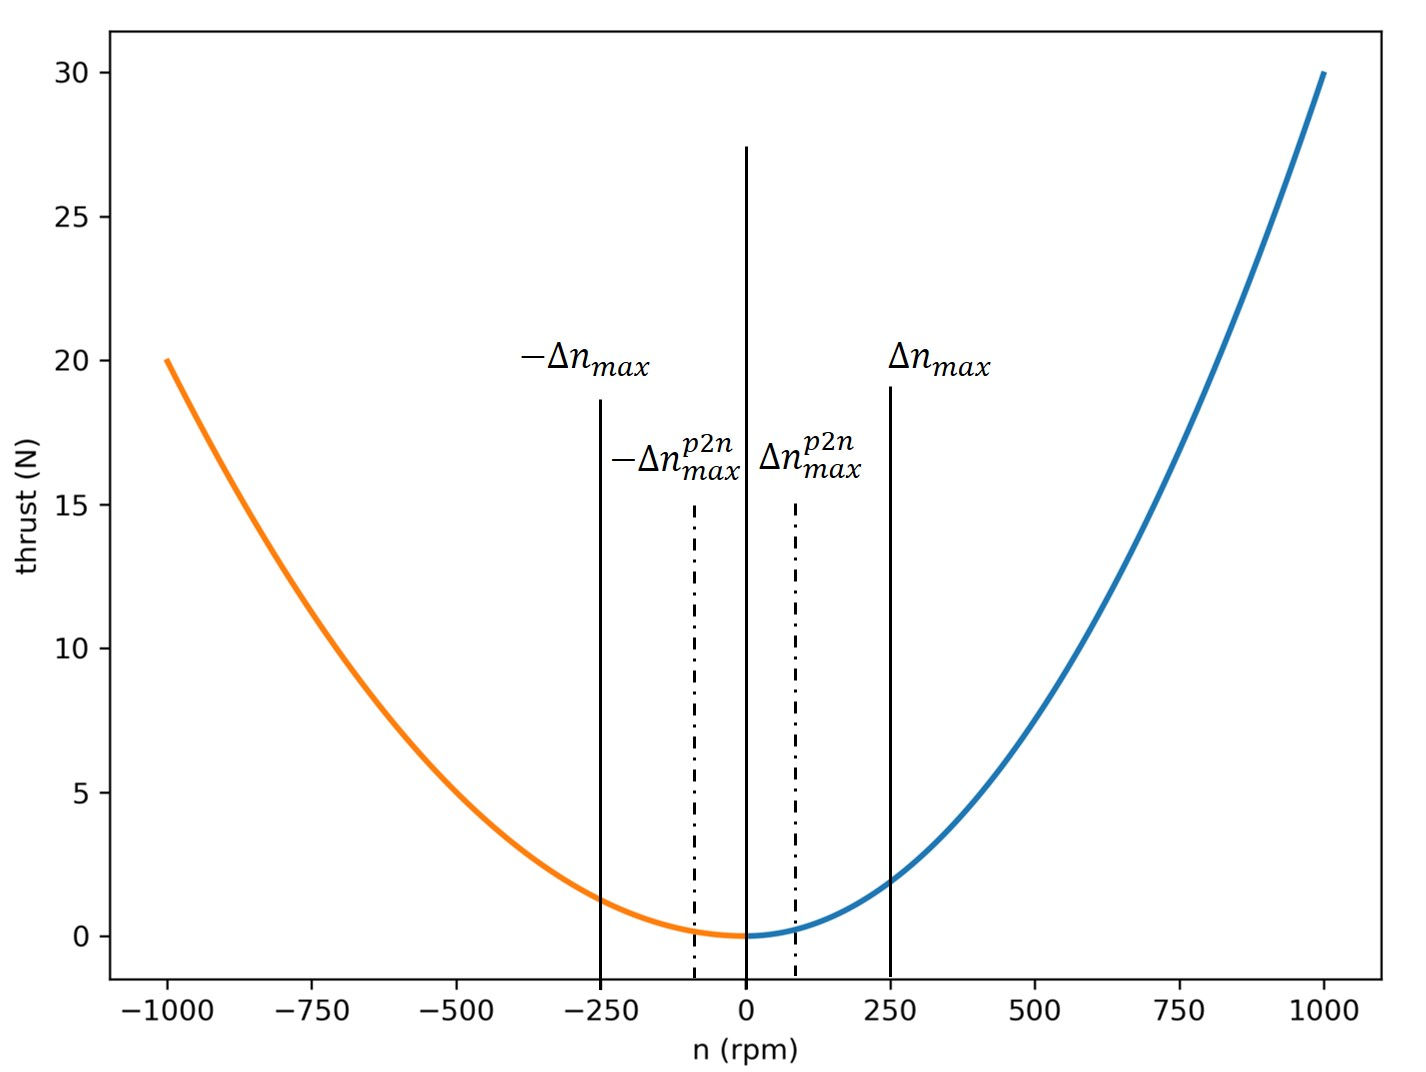
\includegraphics[width=10cm]{chapter02/twinfixed.jpg}
  \bicaption[固定式双尾推螺旋桨的推力曲线]
    {固定式双尾推螺旋桨的推力曲线}
    {Thrust(N) vs. rotational speed (rpm) of Twin fixed thruster}
  \label{fig:twinfixed}
\end{figure}

\begin{figure}[!htp]
  \centering
  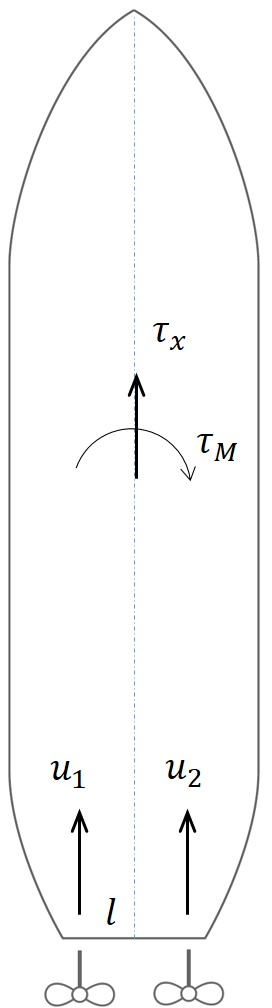
\includegraphics[width=3cm]{chapter02/twinfixed1.jpg}
  \bicaption[固定式双尾推螺旋桨的推力分配]
    {固定式双尾推螺旋桨的推力分配}
    {Thrust allocation of Twin fixed thruster}
  \label{fig:twinfixed1}
\end{figure}

\subsubsection{主推配合船舵}
如图\ref{fig:thrusteralpha}所示,船舵的舵角$\varphi$和其产生推力方向$\alpha$不一致,
他们的关系参见公式(\ref{eq:rudderthrust})。
\begin{equation}
  \begin{aligned}
    &u_x = k n^2 (1- 0.02 C_y \varphi^2) \\
    &u_y = k n^2 C_y \varphi
  \end{aligned}
\end{equation}
由此可得
\begin{equation}
  \begin{aligned}
    &\tan \alpha = \frac{C_y \varphi}{1- 0.02 C_y \varphi^2},  \quad \alpha \in
    [-\frac{\pi}{2}, \, \frac{\pi}{2}] \\
    &u=kn^2 \sqrt{(0.02C_y\varphi^2)^2+(C_y^2 -0.04 C_y)\varphi^2 +1}
  \end{aligned}
\end{equation}
利用$\tan \alpha$的单调性,我们能够计算$\alpha$的约束条件;同时,$u$的极值也可以分别计算
$kn^2$和$(0.02C_y\varphi^2)^2+(C_y^2 -0.04 C_y)\varphi^2 +1$的极值得到。

\subsection{全驱动船}
北东地(North-East-Down: NED)坐标系$\NEDframe=(x_n, y_n, z_n)$是
常用的导航坐标系,通常定义在地球表面的切平面上,其中$x$轴指向地球北,$y$轴指向地球东,
$z$轴垂直于地球表面并指向下。通常对于海上船舶,经纬度的变化并不大,我们可以假定$\NEDframe$
是惯性参考系。

\subsubsection{隧道式艏侧推}
\begin{enumerate}
  \item $n_0 \geq \Delta n_{max}$
  \begin{itemize}
    \item $\underline{\Delta \alpha} = \overline{\Delta \alpha} = 0$
    \item $\overline{\Delta u}= \min \left( u_{max}-k^+ n_0^2 \, , \,
    k^+ (n_0+ \Delta n_{max})^2 - k^+ n_0^2 \right)$
    \item $\underline{\Delta u}=k^+ (n_0 - \Delta n_{max})^2 - k^+ n_0^2 $
  \end{itemize}

  \item $0 < n_0 < \Delta n_{max}$
  \begin{itemize}
    \item if $u_d < 0$
    \begin{itemize}
      \item $\underline{\Delta \alpha} = \overline{\Delta \alpha} = -\pi$
      \item $\overline{\Delta u}= \underline{\Delta u}=
      k^- (n_0 - \Delta n_{max})^2 - k^+ n_0^2$
    \end{itemize}
    \item elseif $u_d \geq 0$
    \begin{itemize}
      \item $\underline{\Delta \alpha} = \overline{\Delta \alpha} = 0$
      \item $\overline{\Delta u}= k^+ (n_0 + \Delta n_{max})^2 - k^+ n_0^2$
      \item $\underline{\Delta u}=- k^+ n_0^2$
    \end{itemize}
  \end{itemize}

  \item $-\Delta n_{max} < n_0 < 0$
  \begin{itemize}
    \item if $u_d > 0$
    \begin{itemize}
      \item $\underline{\Delta \alpha} = \overline{\Delta \alpha} = \pi$
      \item $\overline{\Delta u}=\underline{\Delta u}=  k^+ (n_0 + \Delta n_{max})^2 - k^- n_0^2$
    \end{itemize}
    \item elseif $u_d \leq 0$
    \begin{itemize}
      \item $\underline{\Delta \alpha} = \overline{\Delta \alpha} = 0$
      \item $\overline{\Delta u}= k^- (n_0 - \Delta n_{max})^2 - k^- n_0^2$
      \item $\underline{\Delta u}=- k^- n_0^2$
    \end{itemize}
  \end{itemize}

  \item $n_0 \leq -\Delta n_{max}$
  \begin{itemize}
    \item $\underline{\Delta \alpha} = \overline{\Delta \alpha} = 0$
    \item $\overline{\Delta u}= \min \left( u_{min}-k^- n_0^2 \, , \,
    k^- (n_0 - \Delta n_{max})^2 - k^- n_0^2 \right)$
    \item $\underline{\Delta u}=k^- (n_0 + \Delta n_{max})^2 - k^- n_0^2 $
  \end{itemize}
\end{enumerate}

\section{PID控制器}
PID控制器将位置和速度误差作为输入,计算得到预期的广义力,并通过推力分配算法给出每个推进器
的转速和角度。对于一般的PID控制器,我们定义$e(t) = SP - PV$为误差, 则
\begin{equation}
    u(t)= u_{bias} + K_p e(t)+ \frac{K_I}{\tau_I} \int_0^t e(t) dt + K_d \dot{e}(t)
\end{equation}
其中,$SP$代表设定点(setpoint), $PV$代表实际点。
对于离散情况下,积分项通常为
\begin{equation}
  \sum_{i=n_t - N}^{n_t} e_i(t) \Delta t
\end{equation}
其中,$n_t$代表当前时刻,$N$表示积分长度。
一般而言,对于速度控制,我们通常采用PD控制器,可以减少超调和震荡;对于位置控制,可以用
PI控制器减少静差。

\subsection{动力定位}

\section{轨迹跟踪}

\subsection{视线跟踪法}
视线跟踪法(line of sight)\cite{fossen2003line}是一个路径规划的算法,
最早用于航空航天和导弹制导领域,其主要思路是
根据船的位置计算得到预期的首向角,从而使得船体沿着预期的路径运动。如果我们对船体的前进速度
$u$作反馈控制,即
\begin{equation}
  \lim_{t \rightarrow \infty}\left[u(t)-u_{d}(t)\right]=0
\end{equation}
其中,$u_d$是预期的前进速度。对于LOS, 我们定义$\eta = [s,\, d]^T$,则
\begin{equation}
  \begin{aligned}
      & \bm{R}(\theta_k) =
      \begin{bmatrix}
        \cos \theta_k  & \sin  \theta_k  \\
        -\sin  \theta_k & \cos \theta_k
      \end{bmatrix} \\
      & \eta =\bm{R}(\theta_k)
      \begin{bmatrix}
        x_0 - x_{wp1}\\
        y_0 - y_{wp1}
      \end{bmatrix}
  \end{aligned}
\end{equation}
\begin{equation}
  \begin{aligned}
    &\theta_{los}=\theta_r + \theta_k \\
    &\theta_k=  \arctan \frac{y_{wp2} - y_{wp1} }{ x_{wp2} - x_{wp1}} \\
    & \theta_r = \arcsin \frac{-d}{nL_{pp}}
  \end{aligned}
\end{equation}


\begin{figure}[!htp]
  \centering
  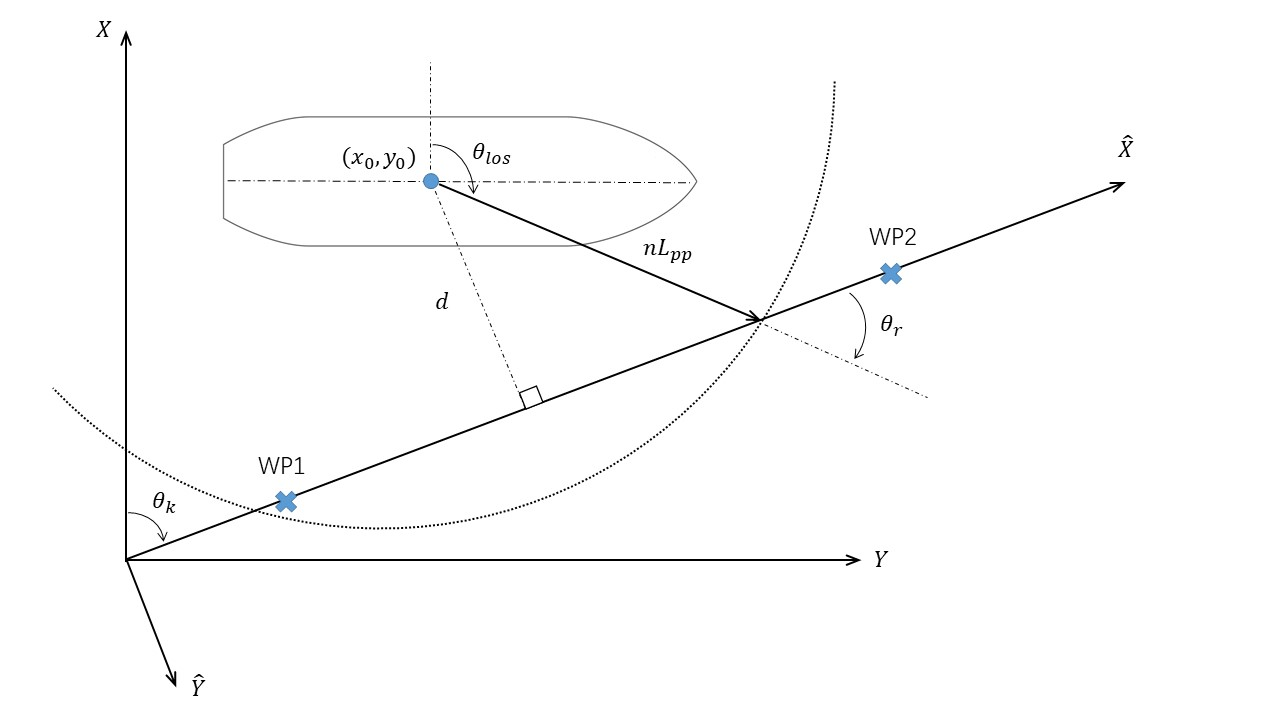
\includegraphics[width=14cm]{chapter02/los.jpg}
  \bicaption[基于视线的轨迹跟踪算法]
    {基于视线的轨迹跟踪算法}
    {Trajectory tracking using line of sight(LOS)}
  \label{fig:lineofsight}
\end{figure}




\section{参数辨识}
\label{sec:parameters}

\chapter{观测器}
\label{chap:chapter03}
\section{移动平均滤波}
简单移动平均(英语:simple moving average,SMA)是某变数之前$n$个数值的未作加权算术平均
\begin{equation}
  \text{SMA}=\frac{p_1+p_2+\cdots + p_n}{n}
\end{equation}
当计算连续的数值,一个新的数值加入,同时一个旧数值剔出,所以无需每次都重新逐个数值加起来:
\begin{equation}
  \text{SMA}_{t1,n}=  \text{SMA}_{t0,n}-\frac{p_1}{n} +\frac{p_{n+1}}{n}
\end{equation}
然而,移动平均滤波的结果存在时滞,当$n$较大时,滤波器产生的结果将不可靠。

\section{卡尔曼滤波}
\subsection{概述}

卡尔曼滤波(Kalman filter)是一种高效率的递归滤波器(自回归滤波器),
它能够从一系列的不完全及包含噪声的测量中,估计动态系统的状态。
卡尔曼滤波会根据各测量量在不同时间下的值,考虑各时间下的联合分布,
再产生对未知变数的估计,因此会比只以单一测量量为基础的估计方式要准。

卡尔曼滤波建立在线性代数和隐马尔可夫模型(hidden Markov model)上。
其基本动态系统可以用一个马尔可夫链表示,该马尔可夫链建立在一个被高斯噪声
(即正态分布的噪声)干扰的线性算子上的。系统的状态可以用一个元素为实数的向量表示。
随着离散时间的每一个增加,这个线性算子就会作用在当前状态上,产生一个新的状态,
并也会带入一些噪声,同时系统的一些已知的控制器的控制信息也会被加入。
同时,另一个受噪声干扰的线性算子产生出这些隐含状态的可见输出。

\subsection{模型}
如图\ref{fig:Basic_concept_of_Kalman_filtering}所示,
为了从一系列有噪声的观察数据中用卡尔曼滤波器估计出被观察过程的内部状态,
必须把这个过程在卡尔曼滤波的框架下建立模型。也就是说对于每一步$k$,
定义矩阵$\bm{F}_k, \bm{H}_k, \bm{Q}_k, \bm{R}_k$,有时也需要定义$\bm{B}_k$,如下。

卡尔曼滤波模型假设$k$时刻的真实状态是从$(k-1)$时刻的状态演化而来,符合下式:
\begin{equation}
  \bm{x}_k=\bm{F}_k \bm{x}_{k-1} + \bm{B}_k \bm{u}_{k} + \bm{w}_k
\end{equation}

其中
\begin{itemize}
  \item $\bm{F}_k$是作用在$\bm{x}_{k-1}$上的状态变换模型(/矩阵/矢量)。
  \item $\bm{B}_k$是作用在控制器向量$\bm{u}_k$上的输入-控制模型。
  \item $\bm{w}_k$是过程噪声,并假定其符合均值为零,协方差矩阵为$\bm{Q}_k$的多元正态分布。
  \item $\bm{w}_{k} \sim N(0 \, , \, \bm{Q}_k)$
\end{itemize}

时刻$k$,对真实状态$\bm{x}_k$的一个测量$\bm{z}_k$满足下式:
\begin{equation}
  \bm{z}_k=\bm{H}_k \bm{x}_k + \bm{v}_k
\end{equation}
其中$\bm{H}_k$是观测模型,它把真实状态空间映射成观测空间,$\bm{v}_k$是观测噪声,
其均值为零,协方差矩阵为$\bm{R}_k$,
且服从正态分布$\bm{v}_{k} \sim N(0 \, , \, \bm{R}_k)$。
初始状态以及每一时刻的噪声${\bm{x}_0, \bm{w}_1, \cdots ,
\bm{w}_k, \bm{v}_1, \cdots \bm{v}_k}$都认为是互相独立的。

实际上,很多真实世界的动态系统都并不确切的符合这个模型;
但是由于卡尔曼滤波器被设计在有噪声的情况下工作,
一个近似的符合已经可以使这个滤波器非常有用了
\begin{figure}[!htp]
  \centering
  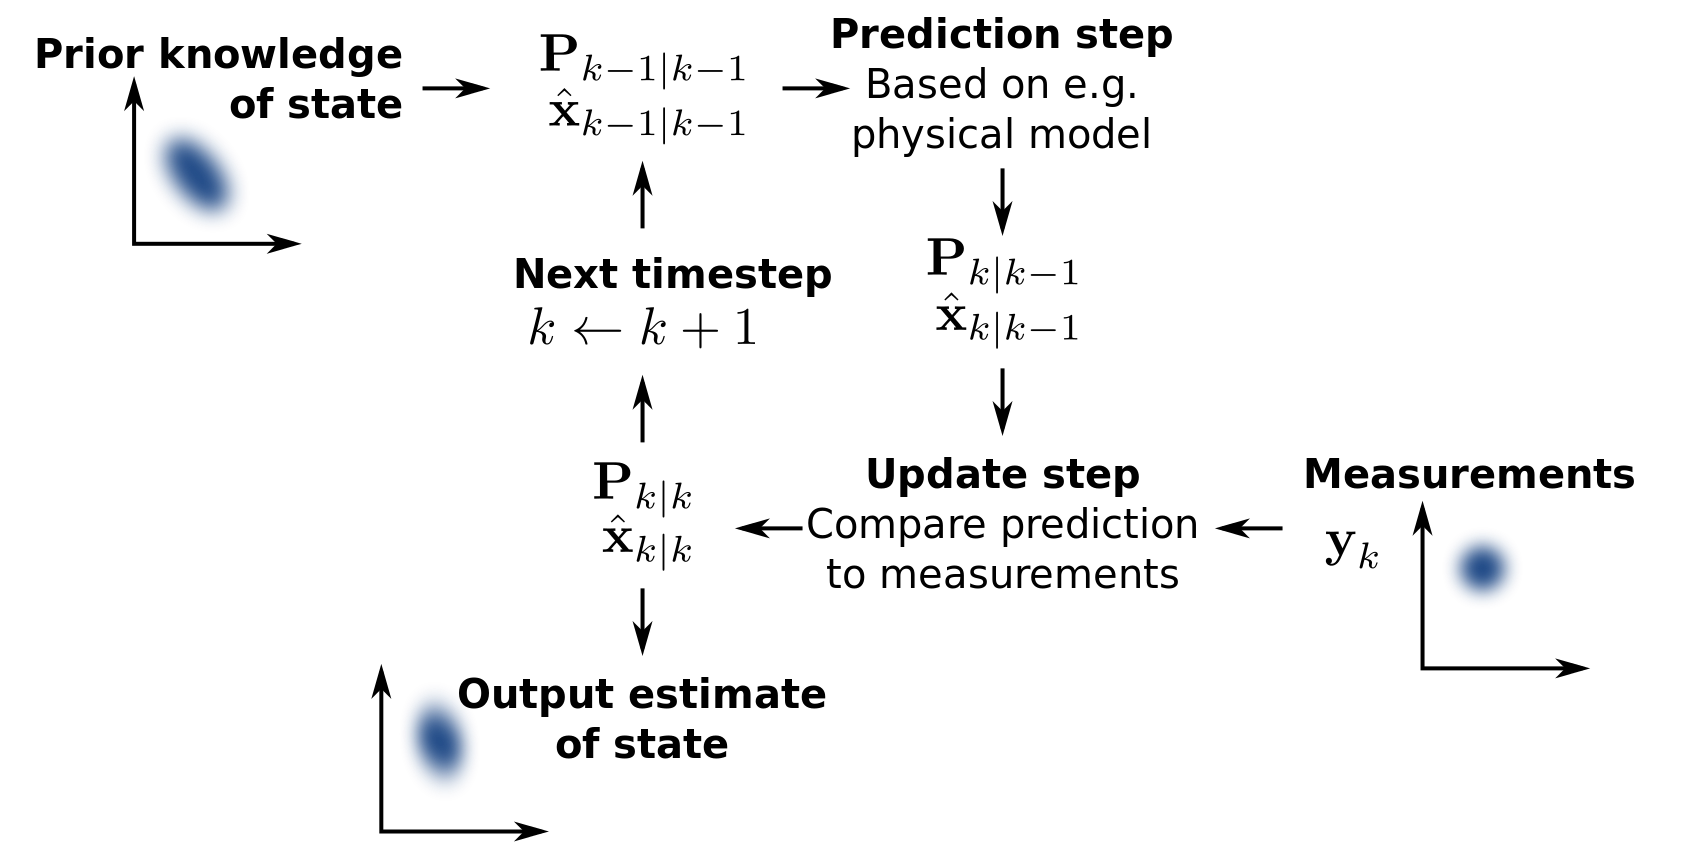
\includegraphics[width=15cm]{chapter03/Basic_concept_of_Kalman_filtering.png}
  \bicaption[卡尔曼滤波的示意图(来自维基百科)]
    {卡尔曼滤波的示意图}
    {The Kalman filter keeps track of the estimated state of the system 
    and the variance or uncertainty of the estimate. 
    The estimate is updated using a state transition model and measurements. 
    $\hat{\bm{x}}_{k \mid k-1}$ denotes the estimate of the system's state 
    at time step $k$ before the $k$-th measurement $\bm{y}_k$ has been 
    taken into account;
    $\bm{P}_{k\mid k-1}$ is the corresponding uncertainty.}
  \label{fig:Basic_concept_of_Kalman_filtering}
\end{figure}

\subsection{算法}
尔曼滤波是一种递归的估计,即只要获知上一时刻状态的估计值以及当前状态的观测值就
可以计算出当前状态的估计值,因此不需要记录观测或者估计的历史信息。
卡尔曼滤波器与大多数滤波器不同之处,在于它是一种纯粹的时域滤波器,
它不需要像低通滤波器等频域滤波器那样,需要在频域设计再转换到时域实现。

卡尔曼滤波器的状态由以下两个变量表示:
\begin{itemize}
  \item $\hat{\bm{x}}_{k | k}$, 在时刻$k$的状态的估计;
  \item $\bm{P}_{k|k}$,后验估计误差协方差矩阵,度量估计值的精确程度。
\end{itemize}

卡尔曼滤波器的操作包括两个阶段:\textbf{预测}与\textbf{更新}。在预测阶段,
滤波器使用上一状态的估计,做出对当前状态的估计。在更新阶段,
滤波器利用对当前状态的观测值优化在预测阶段获得的预测值,以获得一个更精确的新估计值。
\subsubsection{预测}
\begin{equation}
  \begin{aligned}
    &\hat{\bm{x}}_{k|k-1}=\bm{F}_k \hat{\bm{x}}_{k-1 | k-1} + \bm{B}_k \bm{u}_{k} \text{(预测状态)} \\
    &\bm{P}_{k|k-1}=\bm{F}_k \bm{P}_{k-1|k-1} \bm{F}_k^T + \bm{Q}_k
    \text{(预测估计协方差矩阵)}
  \end{aligned}
\end{equation}

\subsubsection{更新}
首先要算出以下三个量:
\begin{equation}
  \begin{aligned}
    &\tilde{\bm{y}}_k = \bm{z}_k - \bm{H}_k \hat{\bm{x}}_{k|k-1}
     \text{(测量余量,measurement residual)} \\
    &\bm{S}_{k}=\bm{H}_k \bm{P}_{k|k-1} \bm{H}_k^T + \bm{R}_k
    \text{(测量余量协方差)} \\
    &\bm{K}_k = \bm{P}_{k|k-1} \bm{H}_k^T \bm{S}_{k}^{-1}
    \text{(最优卡尔曼增益)}
  \end{aligned}
\end{equation}

然后用它们来更新滤波器变量$\bm{x}$与$\bm{P}$:
\begin{equation}
  \begin{aligned}
    &\hat{\bm{x}}_{k|k} = \hat{\bm{x}}_{k|k-1} + \bm{K}_k \tilde{\bm{y}}_k
     \text{(更新的状态估计)} \\
    &\bm{P}_{k|k} =(\bm{I}-  \bm{K}_k \bm{H}_k) \bm{P}_{k|k-1}
    \text{(更新的协方差估计)}
  \end{aligned}
\end{equation}

\subsubsection{不变}
如果模型准确,而且$\hat{\bm{x}}_{0|0}$与$\bm{P}_{0|0}$的值准确的反映了最初状态的分布,
那么以下不变量就保持不变:所有估计的误差均值为零。
\begin{itemize}
  \item $\mathbb{E}[\bm{x}_k - \hat{\bm{x}}_{k|k}] =
      \mathbb{E}[\bm{x}_k - \hat{\bm{x}}_{k|k-1}] = 0$
  \item  $\mathbb{E}[\tilde{\bm{y}}_k]=0$
  \item $\bm{P}_{k|k}= cov(\bm{x}_k - \hat{\bm{x}}_{k|k})$
  \item $\bm{P}_{k|k-1}= cov(\bm{x}_k - \hat{\bm{x}}_{k|k-1})$
  \item $\bm{S}_k = cov(\tilde{\bm{y}}_k)$
\end{itemize}
其中,$\mathbb{E}[a]$表示$a$的期望值,$cov(\bm{a})=\mathbb{E}[\bm{a} \bm{a}^T]$

\subsection{经验}
卡尔曼滤波器中,Q代表Process Noise Covariance Matrix, R代表Measurement Noise
Covariance Matrix; R越小, estimation的结果更"信任"测量值,反之,Q越小,
estimation的结果更"信任"预测值。


\section{GPS天线修正}
由于GPS天线安装的位置不在船体重心处,我们需要对GPS测量结果作修正处理,才能得到重心处的运动。

%# -*- coding: utf-8-unix -*-
% !TEX program = xelatex
% !TEX root = ../thesis.tex
% !TEX encoding = UTF-8 Unicode
%%==================================================
%% chapter02.tex for SJTU Master Thesis
%% based on CASthesis
%% modified by wei.jianwen@gmail.com
%% Encoding: UTF-8
%%==================================================

\chapter{决策与规划}
\label{chap:chapter04}
运动规划(英语:Motion Planning)是一个过程,在考虑运动约束的同时寻找从起始状态到目标状态的移动步骤, 
其整体框架如图\ref{fig:motionplanning}所示 


\begin{figure}[!htp]
  \centering
  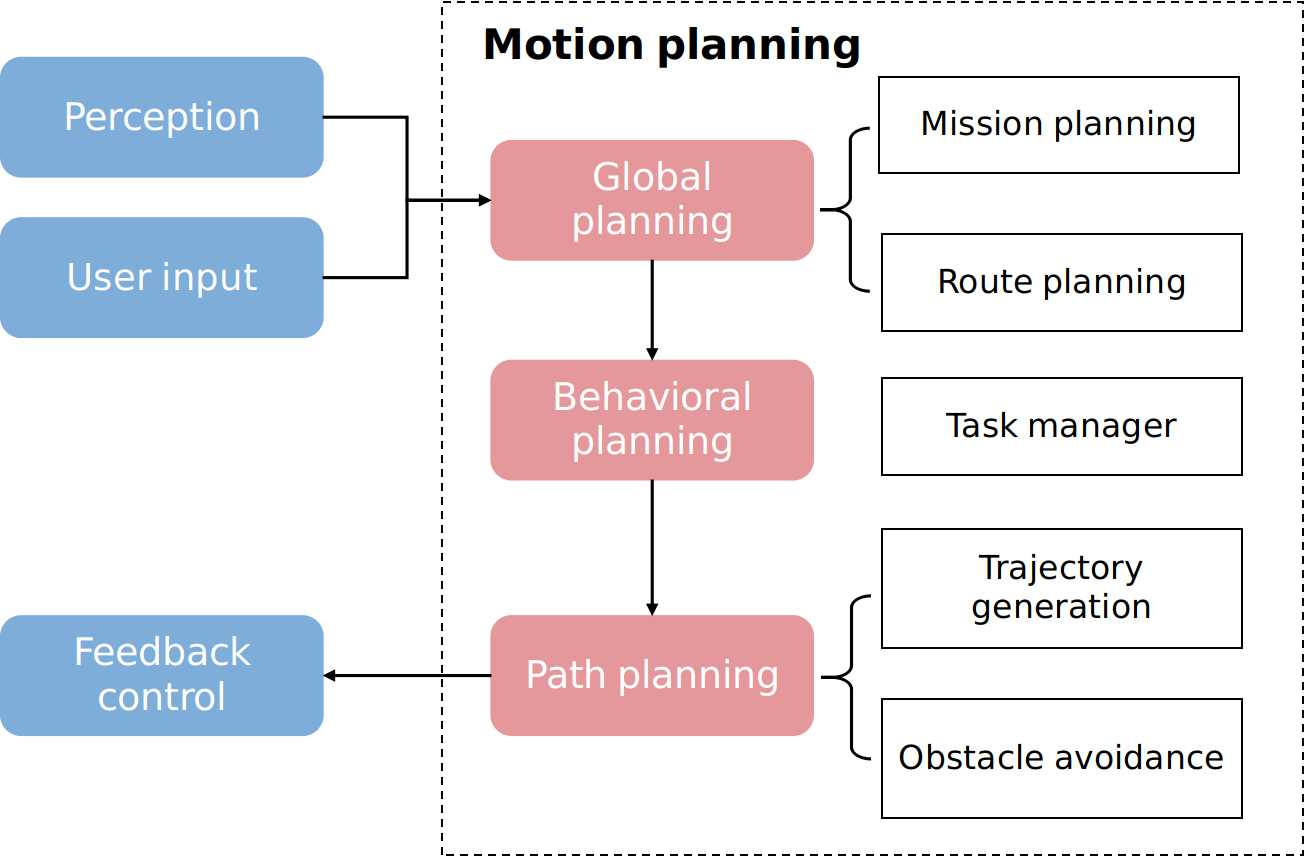
\includegraphics[width=13cm]{chapter04/motionplanning.jpg}
  \bicaption[运动规划的整体框架]
    {运动规划的整体框架}
    {Sketch of motion planning}
  \label{fig:motionplanning}
\end{figure}



\section{路径规划}
\label{sec:pathplanning}

\subsection{航道保持}
航道保持算法是无人船默认的局部路径规划算法, 其适用于中高速航行的船舶,同时可实现多种规划目标
(例如速度保持、超越、跟踪和停止等)。
\subsubsection{Jerk}
\begin{theorem}
\label{thm:jerktheorem}
给定初始时刻$t_0$的初始状态$P_0=[p_0, \dot{p}_0,\ddot{p}_0]$以及结束时刻$t_1= t_0+T$
的状态$P_1=[ \dot{p}_1,\ddot{p}_1]$, 五次多项式是下列惩罚函数的最优解,
\begin{equation}
  \begin{aligned}
    &C=k_j J_t + k_t g(T) + k_p h(p_1) \\
    &J_t(p(t)):=\int_{t_0}^{t_1} \dddot{p}^2(\tau) d \tau
  \end{aligned}
\end{equation}
其中,$g$和$h$是任意函数,$k_j, k_t, k_p>0$, $J_t$(Jerk)通常用于描述加加速度的积分,
其与交通工具的舒适程度有关。
\end{theorem}

\subsubsection{Frenet坐标系}
Frenet坐标系被广泛用于轨迹跟踪和轨迹生成算法中\cite{werling2010optimal}。
在Frenet坐标系中(见图\ref{fig:trajectoryfrenet}),我们以参考轨迹点为原点建立参考坐标系$(\bm{t}_r, \bm{n}_r)$,生成的轨迹点$\bm{x}(s(t),d(t))$可表示为
\begin{equation}
  \label{eq:frenetcoordinate}
  \bm{x}(s(t),d(t)) = \bm{r}(s(t)) + d(t) \cdot \bm{n_r}(s(t))
\end{equation}
表\ref{tab:frenetsymbol}列出了常用的符号,同时我们定义$\dot{(\cdot)}:=
\frac{\partial}{\partial t}(\cdot)$和$(\cdot)':=
\frac{\partial}{\partial s}(\cdot)$

\begin{table}[htbp]
  \centering
  \caption{符号解释}
    \begin{tabular}{ll}
    \toprule
    符号    & 物理含义 \\
    \midrule
    $t$          & 时间 \\
    $T$          & 时间间隔 \\
    $\bm{r}$     & 移动参考坐标系原点(即参考轨迹点)的笛卡尔坐标 \\
    $s$          & 参考轨迹点的弧坐标 \\
    $d$          & 生成轨迹点相对于参考轨迹点的横向偏移量 \\
    $\bm{t}_r$   & 移动参考坐标系的切向量 \\
    $\bm{n}_r$   & 移动参考坐标系的法向量 \\
    $\bm{t}_x$   & 生成轨迹点的切向量 \\
    $\bm{n}_x$   & 生成轨迹点的切向量 \\
    $\bm{x}$     & 生成轨迹的笛卡尔坐标 \\
    $\theta_r$   & 参考轨迹点的方向角 \\
    $\kappa_r$   & 参考轨迹点的曲率 \\
    $\theta_x$   & 生成轨迹点的方向角 \\
    $\kappa_x$   & 生成轨迹点的曲率 \\
    $v_x$  & 生成轨迹点的速度大小 \\
    $a_x$  & 生成轨迹点的加速度大小 \\
    \bottomrule
    \end{tabular}%
  \label{tab:frenetsymbol}%
\end{table}%

\begin{figure}[!htp]
  \centering
  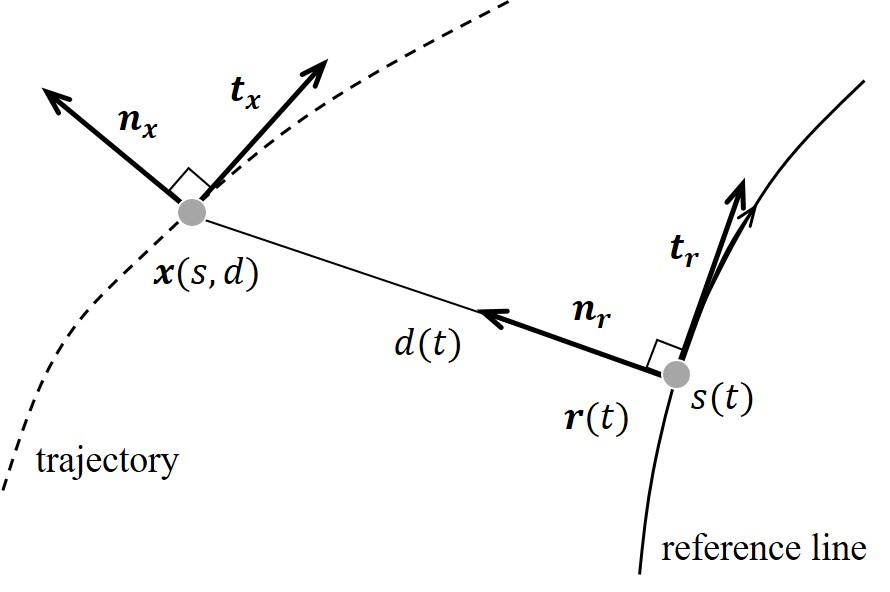
\includegraphics[width=10cm]{chapter04/trajectoryfrenet.jpg}
  \bicaption[Frenet坐标系下的轨迹生成]
    {Frenet坐标系下的轨迹生成}
    {Trajectory generation in a Frenet frame}
  \label{fig:trajectoryfrenet}
\end{figure}

\subsubsection{横向轨迹规划}
\begin{itemize}
  \item \textbf{中高速}

  给定横向的初始状态$D_0=[d_0, \dot{d}_0, \ddot{d}_0]$, 我们假设$\dot{d}_1=\ddot{d}_1=0$
  (这也是我们期望的最终状态),并假设$g(T)=T, \quad h(d_1)=d_1^2$, 由此可得
  \begin{equation}
    C_d = k_j J_t(d(t))+k_t T + k_d d_1^2
  \end{equation}
  $C_d$中最后一项用于惩罚最终状态$d \neq 0$的情况。由定理\ref{thm:jerktheorem}可得,
  $d(t)$是关于$t$的五次多项式(quintic polynomials)。通过调整最终状态的$d_i$和$T_j$
  \begin{equation}
    [d_1,\dot{d}_1,\ddot{d}_1,T]_{ij}=[d_i,0,0,T_j]
  \end{equation}
  注意,船体的状态是实时变化的,因此$D_0$始终表示船体当前时刻的状态,相应的$D_1$表示规划的
  最终状态,也是实时变化的。

  \item \textbf{低速}

  对于中高速的情况下,$s(t)$和$d(t)$可以被分开计算;但对于低速的情况,对$s(t)$和$d(t)$
  独立处理的方法违背了刚体运动的non-holonomic的性质,因此横向轨迹的计算需要考虑纵向轨迹
  \begin{equation}
    \bm{x}(s(t),d(t)) = \bm{r}(s(t)) + d(s(t)) \cdot \bm{n}_r(s(t))
  \end{equation}
  考虑低速的情形,我们修改了惩罚函数
  \begin{equation}
    \begin{aligned}
      &C_d = k_j J_s(d(s)) + k_t S + k_d d_1^2 \\
      &J_s(d(s)):= \int_{s_0}^{s_1} d'''^2(\sigma) d \sigma
    \end{aligned}
  \end{equation}
  该惩罚函数的最优值是$d(s)$关于$s$的五次多项式,且该多项式的初始点$D_0=[d_0, d'_0, d''_0]$
  和终止点为
  \begin{equation}
    [d_1, d'_1,d''_1, T]_{ij}=[d_i, 0, 0, T_j]
  \end{equation}
\end{itemize}

\subsubsection{纵向轨迹规划}
对于纵向的轨迹规划,主要分为跟踪、超越、速度保持和停止。
\begin{itemize}
  \item \textbf{速度保持}

  未感知到障碍物的时候,我们希望船舶匀速航行。结合$s_1$的Transversality condition
  \cite{IROS637936}和定理\ref{thm:jerktheorem},可知四次多项式(quartic polynomials)能够
  使得以下惩罚函数最小,
  \begin{equation}
    C_v = k_j J_t(s(t)) + k_t T + k_{\dot{s}}[\dot{s}_1-\dot{s}_d]^2
  \end{equation}
  其中,我们给定$t_0$时刻$S_0=[s_0, \dot{s}_0, \ddot{s}_0]$,$t_1=t_0+T$时刻的状态
  $S_1=[\dot{s}_1,\ddot{s}_1]$。这就意味着,$s$可以用$t$的四次多项式表示,而多项式的
  初始条件分别为$S_0=[s_0, \dot{s}_0, \ddot{s}_0]$和以下终止条件
  \begin{equation}
    [\dot{s}_1, \ddot{s}_1, T]_{ij}= [\dot{s}_d+\Delta \dot{s}_i, 0, T_j]
  \end{equation}
  当我们调整$\Delta \dot{s}_i$和$T_j$时,可得不同终止条件下的轨迹。
  \item \textbf{跟踪}

  对于跟踪、超越和停止的情况,都存在目标的位置$s_{target}(t)$,给定了$S_0 = [s_0,
  \dot{s}_0, \ddot{s}_0]$和以下的终止条件
  \begin{equation}
    [s_1, \dot{s}_1,\ddot{s}_1, T]_{ij}=[s_{target}(T_j)+\Delta s_i \: ,
    \dot{s}_{target}(T_j) \: , \ddot{s}_{target}(T_j) \: , T_j]
  \end{equation}
  可得$s(t)$关于$t$的五次多项式是以下惩罚函数(cost function)的最优解,
  \begin{equation}
    C_t = k_j J_t + k_t T + k_s(s_1-s_d)^2
  \end{equation}
  当我们调整终止条件中的$\Delta s_i$和$T_j$,可得多条纵向轨迹。

  对于跟踪,也就是与前方的船舶保持一定的距离,这个距离也需要满足海事规范,
  \begin{equation}
    s_{target}(t):=s_{lv}(t)-(D_0+\tau \dot{s}_{lv}(t))
  \end{equation}
  其中,$D_0$和$\tau$是常数,$s_{lv}$和$\dot{s}_{lv}$分别是领导船只沿轨迹线的位置和速度。
  \item \textbf{超越和停止}

  \begin{equation}
    s_{target}(t)=\frac{1}{2}[s_a(t)+s_b(t)]
  \end{equation}
  其中$s_a(t)$和$s_b(t)$分别是周围两条船的位置。对于停止的情况,
  $s_{target}=s_{stop} \, , \, \dot{s}_{target}=0 \, , \, \ddot{s}_{target}=0$
\end{itemize}

\subsubsection{轨迹结合}
通过调整终止条件,我们可得横向和纵向的多项式线束(Lattice),$\Pi_{lat}$和$\Pi_{lon}$,
从而生成轨迹线束$\Pi_{lat} \times \Pi_{lon}$,如图\ref{fig:frenetlattice}所示。在选取
最优轨迹的过程中,我们考虑联合惩罚函数$C_{tot}=k_{lat}C_{lat}+k_{lon}C_{lon}$, 同时保证
生成轨迹与障碍物有一定的安全距离。最终保证避障的条件下,选取最优轨迹。

\begin{figure}[!htp]
  \centering
  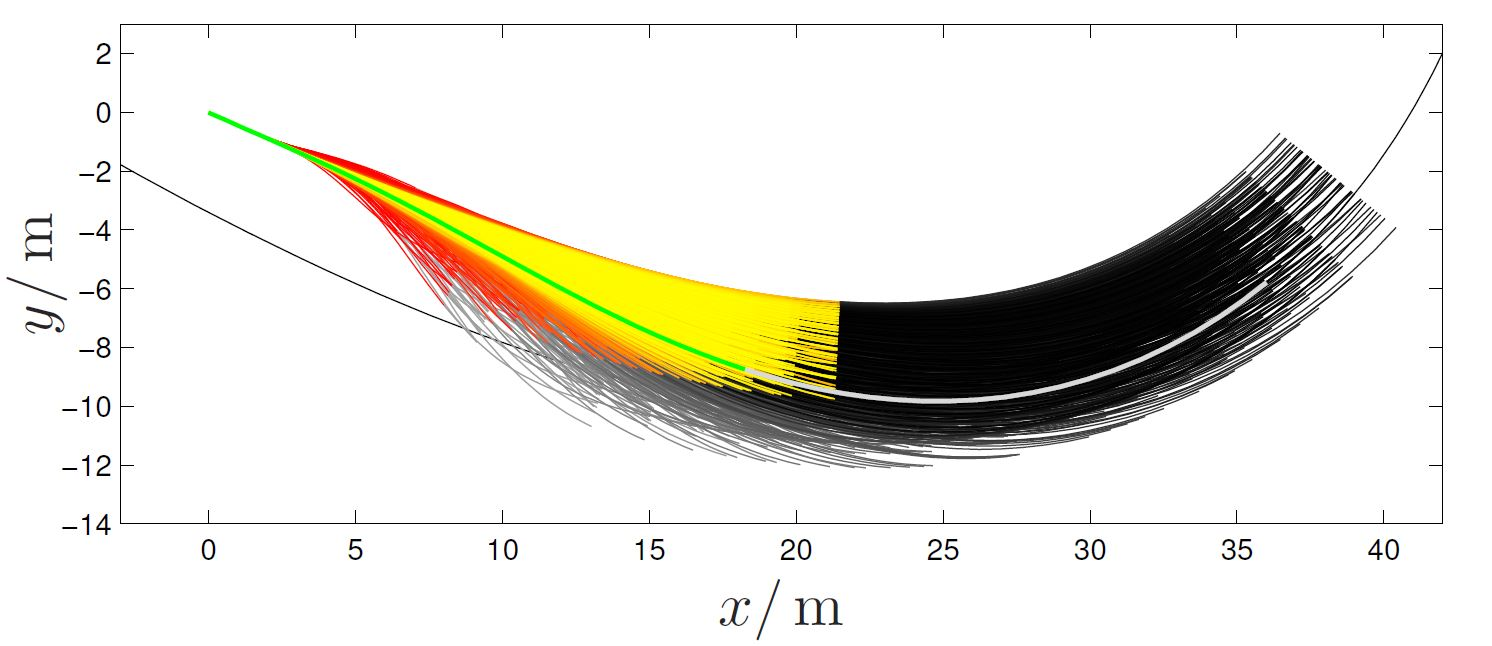
\includegraphics[width=12cm]{chapter04/frenetlattice.jpg}
  \bicaption[Frenet坐标系下的最优轨迹线束]
    {Frenet坐标系下的最优轨迹线束, 其预测时间为3秒,红色到黄色代表递增的惩罚值(cost),
    当障碍物不存在时,“绿-灰”的轨迹即为最优轨迹,使得船体回归参考轨迹。}
    {Resulting trajectory set in global coordinates for velocity keeping: The color map visualizes the increasing costs of both the reactive layer with 3.0 s lookahead from red to yellow and the alternatives for the long-term objectives form gray to black. As there are no obstacles within the 3.0 s horizon, the optimal trajectory of the free problem is chosen (green, light gray), which leads the vehicle back to the center line and to the desired speed.
    }
  \label{fig:frenetlattice}
\end{figure}


\subsubsection{坐标转换}
计算轨迹线束时,需要Frenet坐标系和Cartesian坐标系的相互转换。Frenet坐标系下的船体状态为
$ [s, \dot{s}, \ddot{s} \,; d, \dot{d},\ddot{d}/d, d', d'']$和$[\bm{x}, \theta_x, \kappa_x, v_x, a_x]$,首先我们推导一些通用的公式。

我们定义$\bm{t}_r(s):=[\cos(\theta_r(s)) \: \sin(\theta_r(s))]^T$,
$\bm{n}_r(s):=[ -\sin(\theta_r(s)) \: \cos(\theta_r(s))]^T$和
$\Delta \theta:=\theta_x - \theta_r$,且确保$|\Delta \theta| < \frac{\pi}{2}$和
$1-\kappa_r d >0$。
由Frenet-Serret公式可得
\begin{equation}
  \begin{aligned}
    &\frac{\mathrm{d} \bm{n}_r}{\mathrm{d} s} = -{\kappa}_r \bm{t}_r, \quad
    \frac{\mathrm{d} \bm{n}_r}{\mathrm{d} t} = -\dot{s}{\kappa}_r \bm{t}_r \\
    &\frac{\mathrm{d} \bm{t}_r}{\mathrm{d} s} = {\kappa}_r \bm{n}_r, \quad
    \frac{\mathrm{d} \bm{t}_r}{\mathrm{d} t} = \dot{s} {\kappa}_r \bm{n}_r
  \end{aligned}
\end{equation}
结合Frenet-Serret公式,由方程\ref{eq:frenetcoordinate}可得
\begin{equation}
  d=[\bm{x}-\bm{r}(s)]^T \cdot \bm{n}_r
\end{equation}
对上式作时间的导数,可得
\begin{equation}
  \begin{aligned}
    \dot{d}
    &=[\dot{\bm{x}}-\dot{\bm{r}}(s)]^T \bm{n}_r +
            [\bm{x}-\bm{r}(s)]^T \dot{\bm{n}}_r \\
    &=v_x \bm{t}_x^T \bm{n}_r - \dot{s} \bm{t}_r^T \bm{n}_r - \dot{s} {\kappa}_r
    [\bm{x}-\bm{r}(s)]^T \bm{t}_r \\
    &= v_x \sin(\Delta \theta)
  \end{aligned}
\end{equation}
同时,我们得到
\begin{equation}
  \begin{aligned}
    v_x
    &= || \dot{\bm{x}} ||_2 \\
    &= || \dot{\bm{r}}(s) + \dot{d} \bm{n}_r +d \dot{\bm{n}}_r ||_2 \\
    &= || \dot{s}\bm{t}_r + \dot{d} \bm{n}_r - \dot{s} {\kappa}_r d \bm{t}_r ||_2 \\
    &= \left\|
        \left[
          \begin{array}{cc}
            {\bm{t}_{r}} & {\bm{n}_{r}}
          \end{array}
        \right]
        \left[
          \begin{array}{cc}
            {1-\kappa_{r} d} & {0} \\ {0} & {1}
          \end{array}
        \right]
        \left[
          \begin{array}{c}
            {\dot{s}} \\ {\dot{d}}
          \end{array}
        \right]
      \right\|_2 \\
    &= \sqrt{(1-{\kappa}_r d)^2 \dot{s}^2 +\dot{d}^2}
  \end{aligned}
\end{equation}
且
\begin{equation}
  \label{eq:ddds}
  \begin{aligned}
    d'
    &=\frac{\mathrm{d} t}{\mathrm{d} s} \frac{\mathrm{d} }{\mathrm{d} t} d
    =\frac{\dot{d}}{\dot{s}} = \frac{1}{\dot{s}} v_x \sin(\Delta \theta) \\
    &=\sqrt{(1-{\kappa}_r d)^2 +d'^2}  \sin(\Delta \theta) \\
    & \Rightarrow \\
    d'
    &=(1-{\kappa}_rd) \tan(\Delta \theta)
  \end{aligned}
\end{equation}
已知$(\bm{x}-\bm{r}(s))^T \bm{t}_r = 0$,对其作时间导数可得 $  \frac{v_x}{\dot{s}} \cos(\Delta \theta) -1 + {\kappa}_r d = 0$, 变化得到船体的速度大小
\begin{equation}
  v_x = \dot{s} \frac{1-{\kappa}_r d}{\cos(\Delta \theta)}
\end{equation}
我们用$s_x$表示轨迹$\bm{x}$上的弧长,根据曲率的定义${\kappa_x}=\frac{\mathrm{d} \theta_x}{\mathrm{d}s_x}$和${\kappa_r}=\frac{\mathrm{d} \theta_r}{\mathrm{d}s}$,
可得
\begin{equation}
  \frac{\mathrm{d}}{\mathrm{d}s} =\frac{\mathrm{d} s_x}{\mathrm{d}t}
  \frac{\mathrm{d} t}{\mathrm{d} s} \frac{\mathrm{d}}{\mathrm{d}s_x}
  = \frac{v_x}{\dot{s}} \frac{\mathrm{d}}{\mathrm{d}s_x}
  =\frac{1-{\kappa}_r d}{\cos(\Delta \theta)} \frac{\mathrm{d}}{\mathrm{d}s_x}
\end{equation}
\begin{equation}
  \begin{aligned}
    \Delta \theta ' = \frac{\mathrm{d}( {\theta}_x - {\theta}_r)}{\mathrm{d}s}
    &= \frac{\mathrm{d}}{\mathrm{d} s} {\theta}_x - {\kappa}_r \\
    &= \frac{1-{\kappa}_r d}{\cos(\Delta \theta)} {\kappa}_x - {\kappa}_r  \\
  \end{aligned}
\end{equation}
由公式\ref{eq:ddds},我们可得$d$对$s$的二阶导数
\begin{equation}
  d''=-({\kappa}_r  d)' \tan(\Delta \theta) + \frac{1-{\kappa}_r d}
  {\cos^2(\Delta \theta)}    \Delta \theta '
\end{equation}
将速度$v_x$对时间求导可得
\begin{equation}
  a_x := \dot{v}_x = \ddot{s}\frac{1-{\kappa}_r d}{\cos(\Delta \theta)}  +
  \frac{\dot{s}^2}{\cos(\Delta \theta)}[d' \Delta \theta' - ({\kappa}_r d)']
\end{equation}
同时, $s$对时间$t$的二阶导数
\begin{equation}
  \ddot{s}=\frac{a_x \cos(\Delta \theta)- \dot{s}^2
  [d' \Delta \theta' - ({\kappa}_r d)']}{1-{\kappa}_r d}
\end{equation}
在中高速的情况下($d$与$s$无关),
\begin{equation}
  \begin{aligned}
    &\dot{d}=\frac{\mathrm{d}}{\mathrm{d} t}d=\frac{\mathrm{d}s}{\mathrm{d} t}
    \frac{\mathrm{d}}{\mathrm{d} s}d= \dot{s}d' \\
    &\ddot{d}=d'' \dot{s}^2 + d' \ddot{s}
  \end{aligned}
\end{equation}


坐标系之间的转换将会用于Frenet Lattice的实时计算中(如图\ref{fig:frenetalgorithm}),
下面我们分别讨论两个坐标系之间的转换过程
\begin{itemize}
  \item \textbf{从Cartesian到Frenet}

  给定船体当前时刻的状态为$[\bm{x},\theta_x, \kappa_x, v_x, a_x](t_0)$, 我们希望得到
  在Frenet坐标系下,当前时刻的状态$[s_0, \dot{s}_0, \ddot{s}_0, d_0, \dot{d}_0,
  \ddot{d}_0]$或者$[s_0, \dot{s}_0, \ddot{s}_0, d_0, d'_0, d''_0]$。
  \begin{equation}
    [\bm{x}, \theta_x, \kappa_x, v_x, a_x]  \rightarrow
    [s, \dot{s}, \ddot{s}; d, \dot{d},\ddot{d}/d, d', d'']
  \end{equation}
  首先,采用一些高效的数值方法得到船体在参考轨迹上的投影点$s$
  \begin{equation}
    s= arg\,min_{\sigma} || \bm{x}-\bm{r}(\sigma)||
  \end{equation}
  得到$s$之后,根据参考轨迹的多项式公式,可得${\kappa}_r, {\kappa}'_r$和${\theta}_r$,
  从而计算$\Delta \theta = {\theta}_x-{\theta}_r $, 剩下的变量也可以根据以上公式推导
  得到。

  \item \textbf{从Frenet到Cartesian}

  当我们得到生成轨迹$[s, \dot{s}, \ddot{s}; d, \dot{d},\ddot{d}/d, d', d'']$的时候,
  需要得出Cartesian坐标系中,生成轨迹的状态
  \begin{equation}
    [s, \dot{s}, \ddot{s}; d, \dot{d},\ddot{d}/d, d', d''] \rightarrow
    [\bm{x}, \theta_x, \kappa_x, v_x, a_x]
  \end{equation}

\end{itemize}

\begin{figure}[!htp]
  \centering
  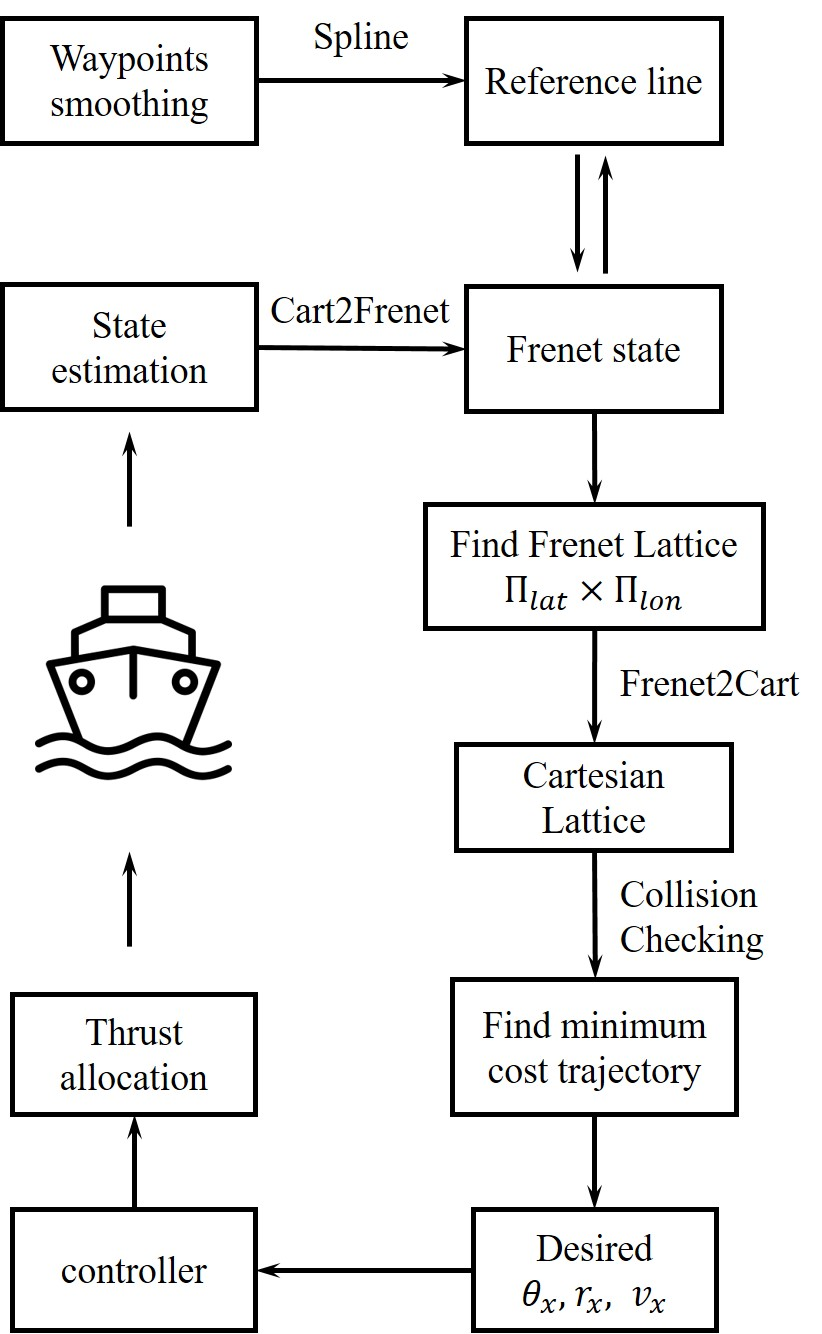
\includegraphics[width=15cm]{chapter04/Algorithm.jpg}
  \bicaption[Frenet坐标系下的最优轨迹生成算法逻辑图]
    {Frenet坐标系下的最优轨迹生成算法逻辑图}
    {Flowchart for trajectory generator in the Frenet frame}
  \label{fig:frenetalgorithm}
\end{figure}


\subsection{低速泊船}
Hybrid A* algorithm
自动停车是一种自动驾驶汽车的系统,它将车辆从行车道移入停车位,以执行平行,垂直或角度停车。

\subsubsection{Reeds-Shepp曲线}
对于欠驱动的机器人(nonholonomic system),其运动模型为

\begin{equation}
  \begin{aligned}
    & x(t)=x(0)+\int_0^t \varepsilon( \tau ) \cos \phi (\tau) d \tau   \\
    & y(t)=y(0)+\int_0^t \varepsilon( \tau ) \sin \phi (\tau) d \tau   \\
    & \phi (t)= \phi (0) + \int_0^t \eta (\tau) d \tau
  \end{aligned}
\end{equation}

其中,$\gamma(t)=[x(t), y(t), \phi(t)]$为机器人的可行轨迹。

如何找到一条最短的路径把船从一个地方开到另外一个地方。答案就是图\ref{fig:rscurve}所示的
Reeds-Shepp曲线\cite{reeds1990} 。
假设车辆能以固定的半径转向,且车辆能够前进和后退,
那么Reeds-Shepp曲线就是车辆在上述条件下从起点到终点的最短路径。
该曲线不仅能保证车辆能够到达终点,而且能保证车辆的角度能在终点到达预期角度。


\begin{figure}[!htp]
  \centering
  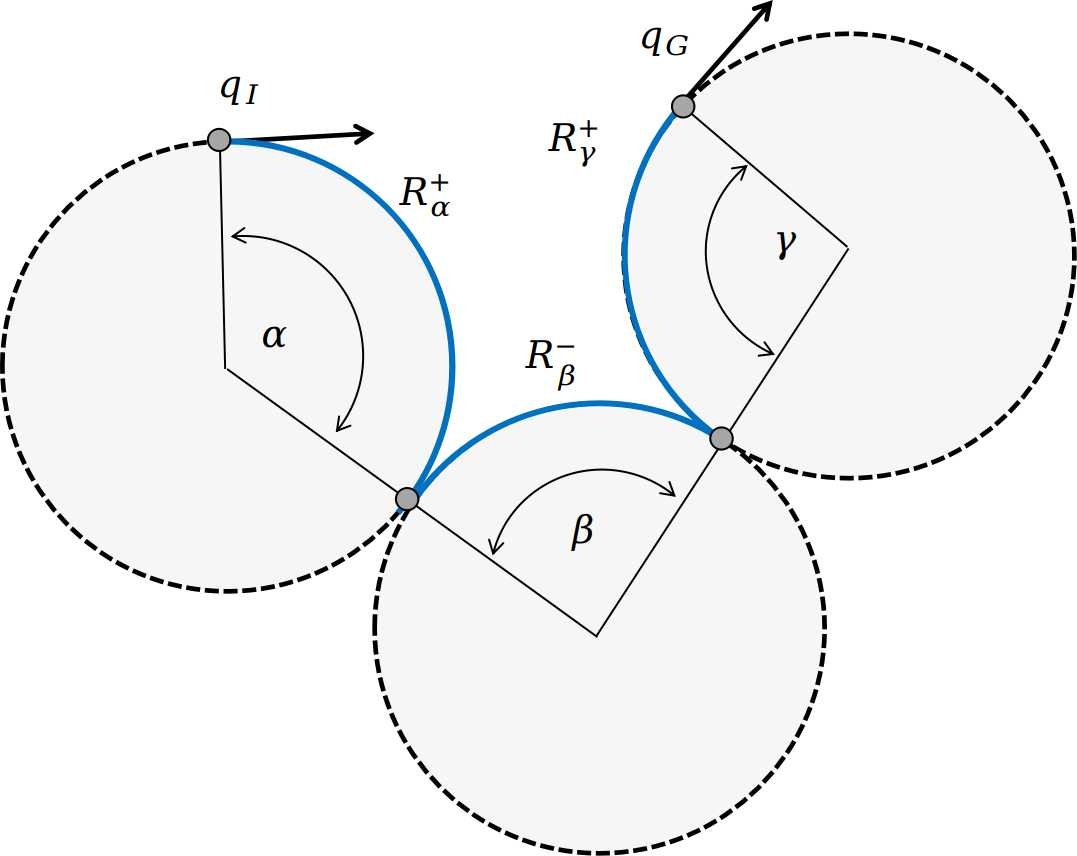
\includegraphics[width=9cm]{chapter04/RScurve.jpg}
  \bicaption[Reeds-Shepp曲线]
    {Reeds-Shepp曲线}
    {An example of Reeds-Shepp curve}
  \label{fig:rscurve}
\end{figure}


\subsubsection{碰撞检测}
我们用矩形包络船体,且用点、线段和最小边框(bounding box)表示周围的物体,
从而通过检测点、线段和最小边框是否与船体矩形重合来检测碰撞。


\subsubsection{A*算法}
A*搜索算法是一种在图形平面上,有多个节点的路径,求出最低通过成本的算法。
用于游戏中的NPC的移动计算,或网络游戏的BOT的移动计算上。
该算法综合了最良优先搜索和Dijkstra算法的优点:在进行启发式搜索提高算法效率的同时,
可以保证找到一条最优路径(基于评估函数)。在此算法中,如果以$g(n)$表示从起点到任意顶点$n$的实际距离,
$h(n)$表示任意顶点$n$到目标顶点的估算距离(根据所采用的评估函数的不同而变化),那么A*算法的估算函数为:

\begin{equation}
  f(n)=g(n)+h(n)
\end{equation}

这个公式遵循以下特性:
\begin{itemize}
  \item 
  如果$g(n)$为0,即只计算任意顶点$n$到目标的评估函数$h(n)$,
  而不计算起点到顶点$n$的距离,则算法转化为使用贪心策略的最良优先搜索,速度最快,但可能得不出最优解;
  \item 
  如果$h(n)$不大于顶点$n$到目标顶点的实际距离,则一定可以求出最优解,
  而且$h(n)$越小,需要计算的节点越多,算法效率越低,常见的评估函数有——欧几里得距离、曼哈顿距离、切比雪夫距离;
  \item 
  如果$h(n)$为0,即只需求出起点到任意顶点$n$的最短路径$g(n)$,而不计算任何评估函数$h(n)$, 
  则转化为单源最短路径问题,即Dijkstra算法,此时需要计算最多的顶点;
\end{itemize}


\subsubsection{轨迹平滑}



\begin{figure}[!htp]
  \centering
  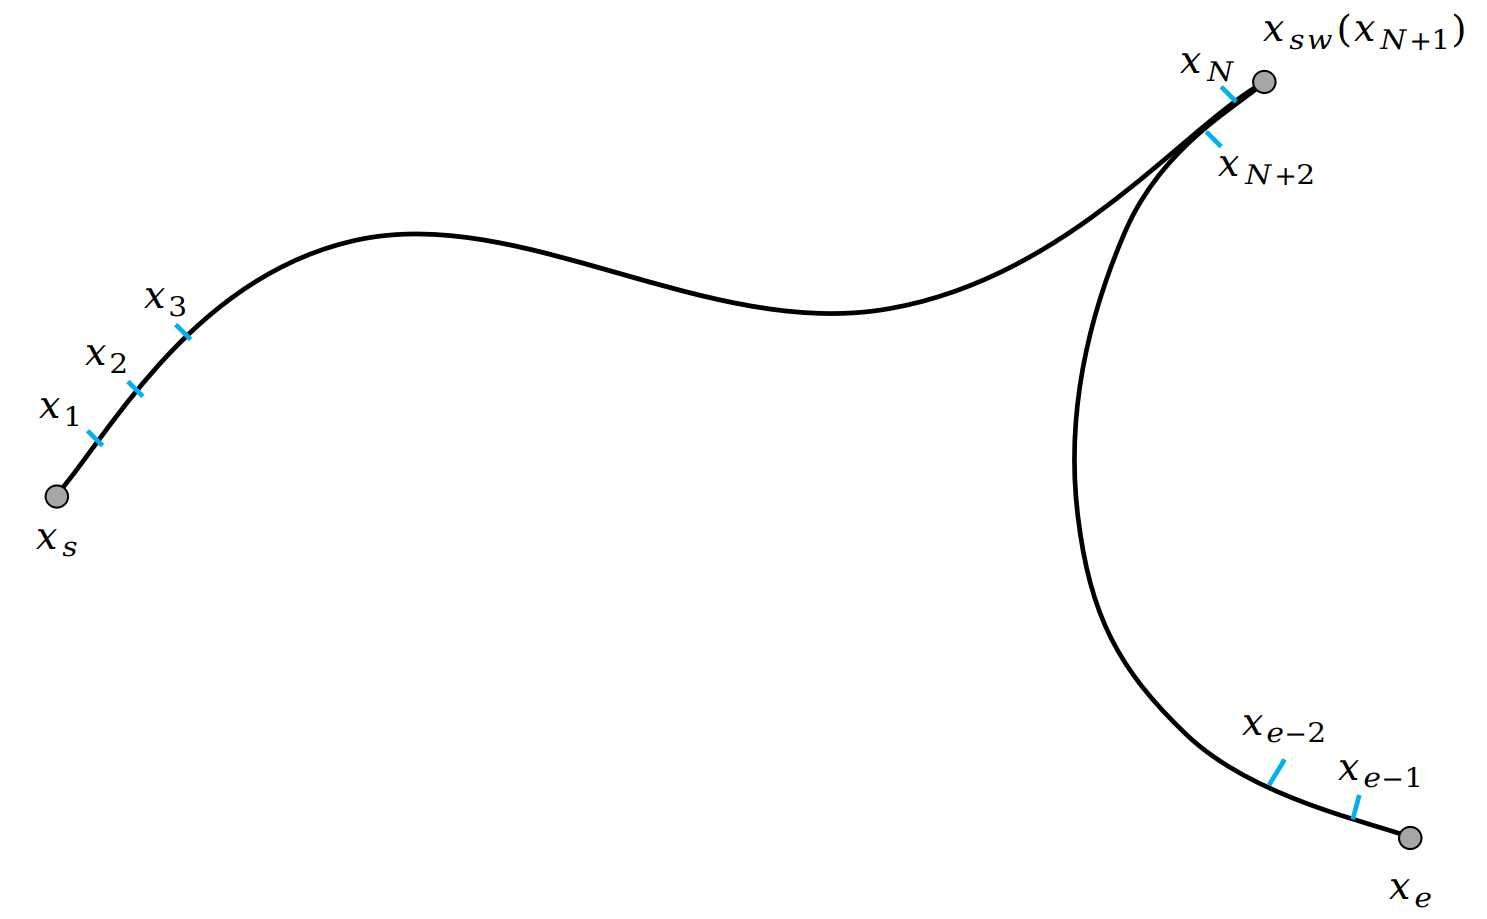
\includegraphics[width=9cm]{chapter04/pathsmoothing.jpg}
  \bicaption[Reeds-Shepp曲线]
    {Reeds-Shepp曲线}
    {An example of Reeds-Shepp curve}
  \label{fig:rscurve}
\end{figure}





\section{航线规划}
\label{sec:routeplanning}

A*算法

\section{行为规划}
\label{sec:behav}

%# -*- coding: utf-8-unix -*-
% !TEX program = xelatex
% !TEX root = ../thesis.tex
% !TEX encoding = UTF-8 Unicode
%%==================================================
%% chapter02.tex for SJTU Master Thesis
%% based on CASthesis
%% modified by wei.jianwen@gmail.com
%% Encoding: UTF-8
%%==================================================

\chapter{环境感知}
\label{chap:chapter05}

\section{航海雷达}
\label{sec:marineradar}

\subsection{SDK}
本节介绍一些常用航海雷达(e.g. SIMRAD 4G)的SDK,以及一些使用注意事项
\subsection{目标跟踪}
\subsubsection{坐标投影}
如图\ref{fig:Radar_spoke_projection}所示,我们用$\theta$表示船体的首向角,
$\theta_s$表示线束的方位角,$\overrightarrow{GR}=
(x_r \, , \,  y_r)$表示航海雷达在船上的位置。
在随体坐标系中,$\overrightarrow{GS}=
(x_r+\rho \cos \theta_s \, , \, y_r+\rho \sin \theta_s )$; 则在全局坐标系下,线束的
的位置可表示如下
\begin{equation}
  \begin{bmatrix}
    x_s \\
    y_s
  \end{bmatrix}=
  \begin{bmatrix}
    \cos \theta & -\sin \theta \\
    \sin \theta & \cos \theta
  \end{bmatrix}
  \begin{bmatrix}
    x_r + \rho \cos \theta_s \\
    y_r + \rho \sin \theta_s
  \end{bmatrix} +
  \begin{bmatrix}
    x_G \\
    y_G
  \end{bmatrix}
\end{equation}

\begin{figure}[!htp]
  \centering
  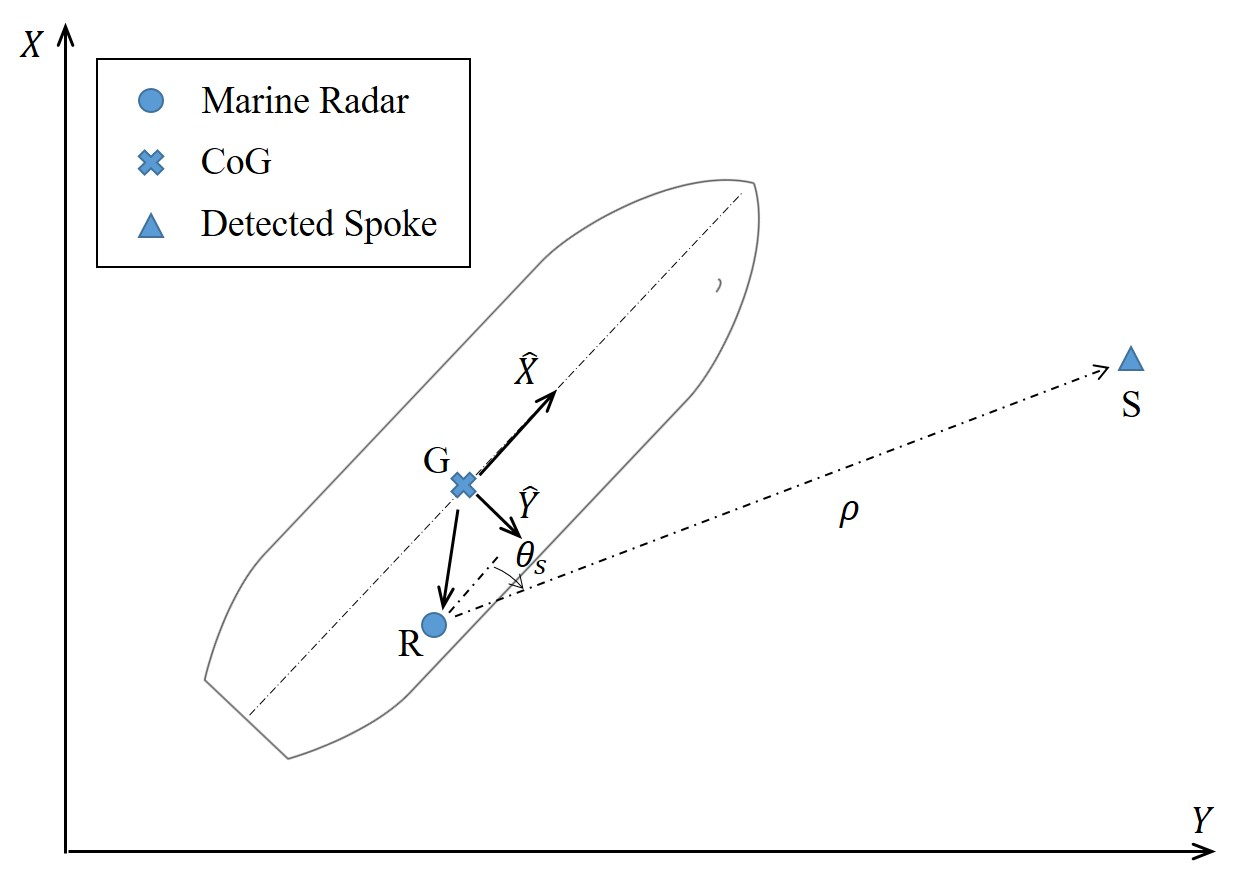
\includegraphics[width=12cm]{chapter05/Radar_spoke_projection.jpg}
  \bicaption[雷达线束的坐标投影]
    {雷达线束的坐标投影}
    {The coordinate projection of spoke data from marine radar}
  \label{fig:Radar_spoke_projection}
\end{figure}

\subsubsection{分类 Clustering}

\subsubsection{包络 Miniball}

\subsubsection{识别 Identification}
当我们得到发现的目标时(Detected targets),需要识别这些目标,
我们用以下符号表示
\begin{itemize}
    \item $\bm{V_{j0}}$: the previous velocity vector of $j$th tracking target
    \item $\bm{V_{ji}}$: The predicted velocity vector of $j$th tracking target
                        when applying the new position of $i$th detected target
    \item $R_D^i$: the radius of $i$th detected target
    \item $R_T^j$: the radius of $j$th tracking target
    \item $V_T$: the speed threhold of targets
\end{itemize}

对于跟踪中的目标$j$,他们是acquiring或acquired, 我们可以

当$|\bm{V_{j0}}| \leq V_T$
\begin{equation}
  \text{Loss}=k_R \frac{|{R_D^i}^2-{R_T^j}^2|}{{R_T^j}^2} +
            k_V \frac{|\bm{V_{j0}}-\bm{V_{ji}}|}{|\bm{V_{j0}}|}
\end{equation}
For loop $i$ in detected targets:

\quad If $|\bm{V_{ji}}|>V_{max}$, continue;

\quad If $|\bm{V_{j0}}-\bm{V_{ji}}|>a_{max} \Delta T$, continue;

find the min Loss;

当$|\bm{V_{j0}}| > V_T$
\begin{equation}
  \text{Loss}=k_R \frac{|{R_D^i}^2-{R_T^j}^2|}{{R_T^j}^2} +
            k_V \frac{|\bm{V_{j0}}-\bm{V_{ji}}|}{|\bm{V_{j0}}|}  +
            k_A \frac{|\angle (\bm{V_{j0}}, \bm{V_{ji}})|}{\pi}
\end{equation}
For loop $i$ in detected targets:

\quad If $|\bm{V_{ji}}|>V_{max}$, continue;

\quad If $|\bm{V_{j0}}-\bm{V_{ji}}|>a_{max} \Delta T$, continue;

\quad If $|\angle(\bm{V_{j0}},\bm{V_{ji}})|>{\alpha}_{max} \Delta T$, continue;

find the min Loss;

The identification for $j$ tracking target, return the matched index in the
detected targets, or return -1 if un-matched.

\subsubsection{$\alpha-\beta$滤波}
$\alpha-\beta$滤波器是一种线性状态观测器,可用于观测刚体运动的位置和速度。当我们假设
在一段时间内$\Delta T$物体的速度是恒定不变的,则
\begin{equation}
  \begin{aligned}
    &\hat{\bm{x}}_k = \hat{\bm{x}}_{k-1} + \Delta T \hat{\bm{v}}_{k-1} \\
    &\hat{\bm{v}}_k = \hat{\bm{v}}_{k-1}
  \end{aligned}
\end{equation}

\section{计算机视觉}


\section{激光雷达}

%# -*- coding: utf-8-unix -*-
% !TEX program = xelatex
% !TEX root = ../thesis.tex
% !TEX encoding = UTF-8 Unicode
\chapter{传感器}
\label{chap:sensor}
\section{全球定位系统}
全球定位系统(Global Positioning System,GPS)是一种以空中卫星为基础的高精度无线电导航的定位系统,
它在全球任何地方以及近地空间都能够提供准确的地理位置、刚体速度及精确的时间信息。
对于室外定位,一般采用GPS或者北斗定位系统。


\subsection{GPS定位定向天线 Hemisphere V102}
Hemisphere V102提供定向、定位、起伏、横滚和俯仰信息,可利用SBAS差分GPS定位,水平精度为
0.5 m; 侧向精度为$0.75^{\circ}$, 俯仰/横滚精度为$1.5^{\circ}$。
使用时推荐采样频率10 Hz, 波特率为115200。
在串口助手里面(cutecom或者sscom)可输入指令(见表\ref{tab:V102command}),
修改V102输出的内容。由于V102不支持北斗功能,与北斗相关的命令是无效的。
每次设置完GPS之后,记得\$JSAVE保存配置


% Table generated by Excel2LaTeX from sheet 'Sheet1'
\begin{table}[htbp]
  \centering
  \caption{Hemisphere V102常用指令}
    \begin{tabular}{p{11.54em}p{19.96em}}
    \toprule
    命令    & 功能 \\
    \midrule
    \$JSHOW & 查询V102的设置 \\
    \$JDIFF & 查询当前差分模式 \\
    \$JDIFF, INCLUDE, SBAS & 设置SBAS参与差分定位 \\
    \$JBAUD, X & 设置当前串口波特率为X, 推荐X=115200 \\
    \$JASC, GPGGA, X & 设置NMEA GPGGA消息的输出频率为 X Hz; 若X=0, 不输出GPGGA的数据;推荐X=10 \\
    \$JASC, GPGSV, X & 设置NMEA GPGSV消息的输出频率为 X Hz \\
    \$JASC, GPHDT, X & 设置NMEA GPHDT消息的输出频率为 X Hz \\
    \$JASC, GPHPR, X & 设置NMEA GPGSV消息的输出频率为 X Hz \\
    \$JASC,GPROT,X & 首向速度(deg/min) \\
    \$JASC, PSAT,ATTSTAT, X & 打开副天线卫星信息,同时包含基线长等信息 \\
    \$JASC, PVCT, X & 输出主副天线的东向,北向,及天向的差值 \\
    \$JATT,GYROAID,YES & 打开陀螺 \\
    \$JATT,GYROAID & 查询陀螺当前状态 \\
    \$JATT,TILTAID,YES & 打开倾斜传感器 \\
    \$JATT,TILTAID & 查询当前倾斜传感器的状态 \\
    \bottomrule
    \end{tabular}%
  \label{tab:V102command}%
\end{table}%

% Table generated by Excel2LaTeX from sheet 'Sheet1'
\begin{table}[htbp]
  \centering
  \caption{防水接头接线方法}
    \begin{tabular}{lp{3.25em}lp{19.25em}}
    \toprule
    \multicolumn{1}{p{3.125em}}{Pin} & 颜色    & \multicolumn{1}{p{3.29em}}{Pin(*)} & 功能 \\
    \midrule
    1     & 白     & 1     & Port C, RS-232 female DB9 pin 2, device out \\
    2     & 绿     & 3     & Port C, RS-232 female DB9 pin 3, device in \\
    5     & 红     & 5     & Power input \\
    7     & 黄     & 2     & Signal Ground \\
    8     & 棕     & 7     & Port A, RS-232 female DB9 pin 3, device in \\
    9     & 蓝     & 6     & Port A, RS-232 female DB9 pin 2, device out \\
    10    & 黑     & 4     & Power Ground \\
    11    & Drain  & 8     & CH\_GND \\
    \bottomrule
    \end{tabular}%
    \begin{tablenotes}
        \footnotesize
        \item[*] 注: Pin指的是V102上的12芯防水接头上的数字,Pin(*)指的是控制盒上
        8芯防水接头上的数字;在控制盒中,Signal Ground一分为二,黄色和灰色线共用。
    \end{tablenotes}
  \label{tab:pluginconnect}%
\end{table}%


\subsection{墨卡托投影}
墨卡托投影,是正轴等角圆柱投影。由荷兰地图学家墨卡托(G.Mercator)于1569年创立。
假想一个与地轴方向一致的圆柱切或割于地球,按等角条件,将经纬网投影到圆柱面上,
将圆柱面展为平面后,即得本投影。墨卡托投影在切圆柱投影与割圆柱投影中,
最早也是最常用的是切圆柱投影。
首先,我们来了解一些常用的导航坐标系
\begin{itemize}
  \item 地理坐标系(Geographic coordinates)地理坐标系一般是指由经度、纬度和相对高度组成
  的坐标系,能够标示地球上的任何一个位置。
  \item 通用横轴墨卡托投影(Universal Transverse Mercator,简称UTM) \cite{hager1989universal} 是一种国际标准化的地图投影法。它使用笛卡尔坐标系,
  标记南纬$80^{\circ}$至北纬$84^{\circ}$之间的所有位置。本坐标系采用WGS84系统作为坐标基础。
  \item 通用极立体坐标系(Universal polar stereographic coordinate system,简称UPS)作为
  UTM的补充,标记南纬$80^{\circ}$以南和北纬$84^{\circ}$以北的所有位置,以及与UTM有$0.5^{\circ}$的重叠。
\end{itemize}

值得注意的是,跨越UTM区域的时候会出现坐标不连续的问题。这里我们在UTM区域之间
引入100公里(100 km)的重叠区(如图\ref{fig:utmoverlap}),从而解决坐标不连续的问题。同时,
在路径规划算法中,用户输入的坐标点需要经过计算,确保Waypoints或者DP setpoint在同一个
UTM区域且不超过100km。

\begin{figure}[!htp]
  \centering
  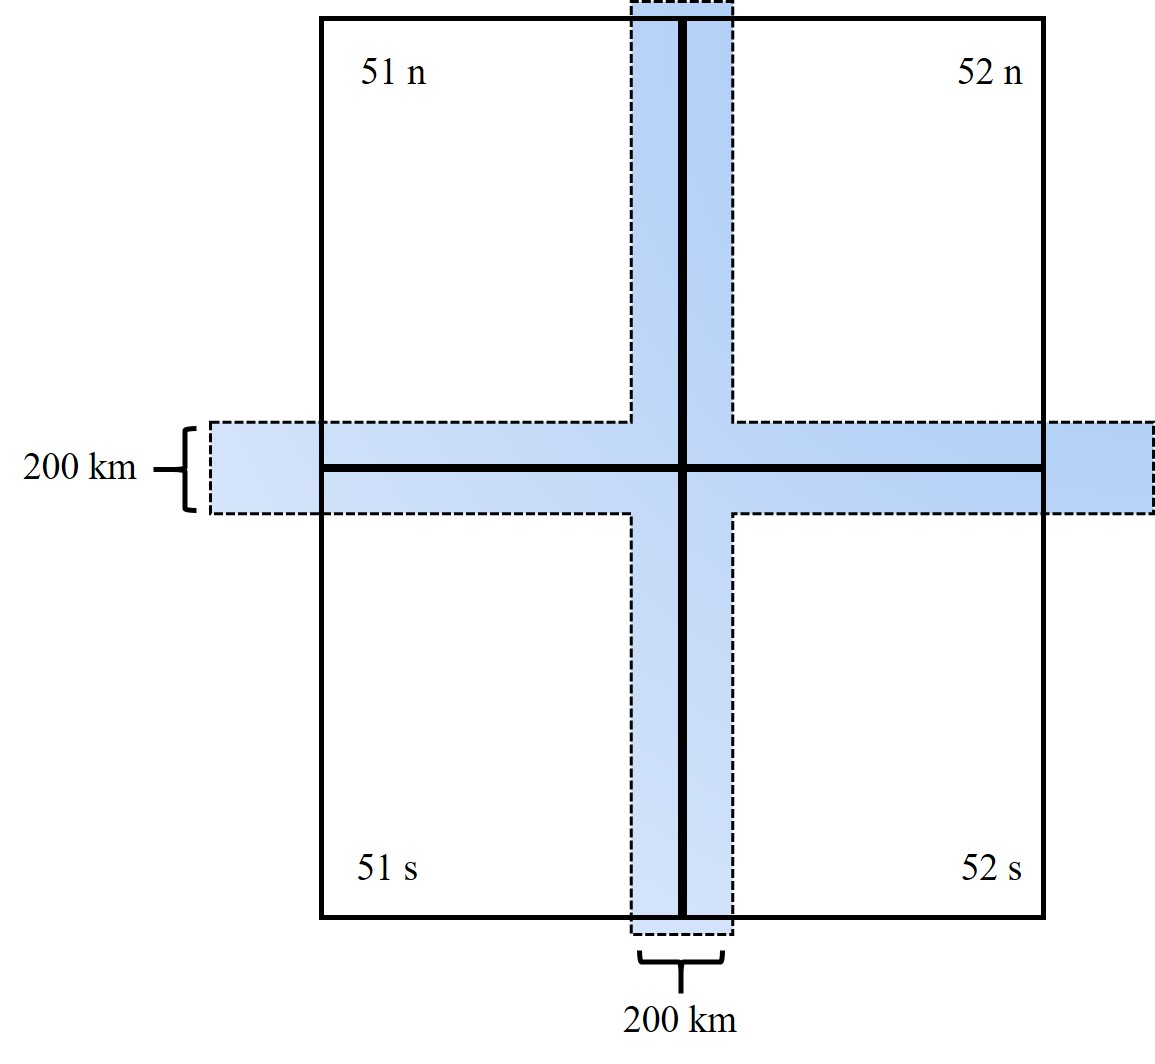
\includegraphics[width=10cm]{chapter_sensor/utmoverlap.jpg}
  \bicaption[UTM区域的重叠]
    {UTM区域的重叠}
    {The overlap between UTM zones}
  \label{fig:utmoverlap}
\end{figure}


\section{惯性测量单元}
惯性测量单元(Inertial measurement unit,简称IMU是测量物体三轴姿态角(或角速率)以及加速度的装置。

\section{航海雷达}
\section{红外热像仪}
\section{风速风向仪}

%# -*- coding: utf-8-unix -*-
% !TEX program = xelatex
% !TEX root = ../thesis.tex
% !TEX encoding = UTF-8 Unicode
%%==================================================
%% chapter02.tex for SJTU Master Thesis
%% based on CASthesis
%% modified by wei.jianwen@gmail.com
%% Encoding: UTF-8
%%==================================================

\chapter{系统架构}
\label{chap:chapter06}

\section{软件系统架构}
\label{sec:marineradar}

\section{电气系统架构}



\subsection{SDK}

% !TeX root = ../thesis.tex

\chapter{浮动体}

\section{插图}

插图功能是利用 \TeX\ 的特定编译程序提供的机制实现的,不同的编译程序支持不同的图
形方式。有的同学可能听说“\LaTeX\ 只支持 EPS”,事实上这种说法是不准确的。\XeTeX
可以很方便地插入 EPS、PDF、PNG、JPEG 格式的图片。

一般图形都是处在浮动环境中。之所以称为浮动是指最终排版效果图形的位置不一定与源文
件中的位置对应,这也是刚使用 \LaTeX\ 同学可能遇到的问题。如果要强制固定浮动图形
的位置,请使用 \pkg{float} 宏包,它提供了 \texttt{[H]} 参数。

\subsection{单个图形}

图要有图题,研究生图题采用中英文对照,并置于图的编号之后,图的编号和图题应置于图
下方的居中位置。引用图应在图题右上角标出文献来源。当插图中组成部件由数字或字母等
编号表示时,可在插图下方添加图注进行说明,如图~\ref{fig:cn_100t} 所示。

\begin{figure}[!htp]
  \centering
  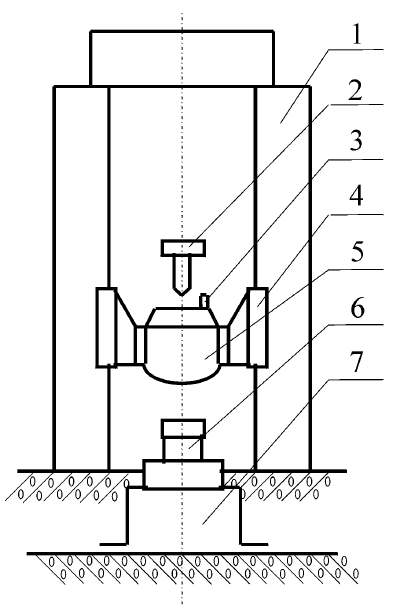
\includegraphics[width=4cm]{cn_100t.png} \\
    1.立柱 2.提升释放机构 3.标准冲击加速度计 \\
    4.导轨 5.重锤 6.被校力传感器 7.底座 \\
  \bicaption[出现在插图索引中]
    {单个图形示例\cite{he1999}。如果表格的标题很长,那么在表格索引中就会很不美观。可
      以在前面用中括号写一个简短的标题,这个标题会出现在索引中。}
    {Stay hungry, stay foolish.}
 \label{fig:cn_100t}
\end{figure}

Lorem ipsum dolor sit amet, consectetur adipisici elit, sed do eiusmod tempor
incididunt ut labore et dolore magna aliqua. Ut enim ad minim veniam, quis
nostrud exercitation ullamco laboris nisi ut aliquip ex ea commodo consequat.
Duis aute irure dolor in reprehenderit in voluptate velit esse cillum dolore eu
fugiat nulla pariatur. Excepteur sint occaecat cupidatat non proident, sunt in
culpa qui officia deserunt mollit anim id est laborum.

\subsection{多个图形}

简单插入多个图形的例子如图~\ref{fig:SRR} 所示。这两个水平并列放置的子图共用一个
图形计数器,没有各自的子图题。

\begin{figure}[!htp]
  \centering
  
\includegraphics[height=2cm]{./pdf/sjtu-badge.pdf}
  \hspace{1cm}
  
\includegraphics[height=2cm]{./pdf/sjtu-badge.pdf}
  \bicaption{中文题图}{English caption}
  \label{fig:SRR}
\end{figure}

如果多个图形相互独立,并不共用一个图形计数器,那么用 \texttt{minipage} 或者
\texttt{parbox} 就可以,如图~\ref{fig:parallel1} 与图~\ref{fig:parallel2}。

\begin{figure}[!htp]
\begin{minipage}{0.48\textwidth}
  \centering
  
\includegraphics[height=1.5cm]{./pdf/sjtu-name.pdf}
  \caption{并排第一个图}
  \label{fig:parallel1}
\end{minipage}\hfill
\begin{minipage}{0.48\textwidth}
  \centering
  
\includegraphics[height=1.5cm]{./pdf/sjtu-name.pdf}
  \caption{并排第二个图}
  \label{fig:parallel2}
\end{minipage}
\end{figure}

Lorem ipsum dolor sit amet, consectetur adipisici elit, sed do eiusmod tempor
incididunt ut labore et dolore magna aliqua. Ut enim ad minim veniam, quis
nostrud exercitation ullamco laboris nisi ut aliquip ex ea commodo consequat.
Duis aute irure dolor in reprehenderit in voluptate velit esse cillum dolore eu
fugiat nulla pariatur. Excepteur sint occaecat cupidatat non proident, sunt in
culpa qui officia deserunt mollit anim id est laborum.

如果要为共用一个计数器的多个子图添加子图题,建议使用较新的 \pkg{subcaption}宏
包,不建议使用 \pkg{subfigure} 或 \pkg{subfig} 等宏包。

推荐使用 \pkg{subcaption} 宏包的 \cs{subcaptionbox} 并排子图,子图题置于子图之
下,子图号用 a)、b) 等表示。也可以使用 \pkg{subcaption} 宏包的 \cs{subcaption}
(放在 minipage中,用法同 \cs{caption})。

搭配 \pkg{bicaption} 宏包时,可以启用 \cs{subcaptionbox} 和 \cs{subcaption} 的双
语变种 \cs{bisubcaptionbox} 和 \cs{bisubcaption},如图~\ref{fig:bisubcaptionbox}
所示。

\begin{figure}[!hbtp]
  \centering
  \bisubcaptionbox{$R_3 = 1.5\text{mm}$ 时轴承的压力分布云图}%
                  {Pressure contour of bearing when $R_3 = 1.5\text{mm}$}%
                  [6.4cm]{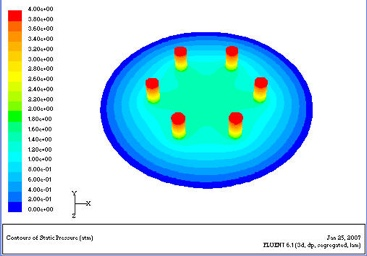
\includegraphics[height=2.5cm]{pressure15.jpg}}
  \hspace{1cm}
  \bisubcaptionbox{$R_3 = 2.5\text{mm}$ 时轴承的压力分布云图}%
                  {Pressure contour of bearing when $R_3 = 2.5\text{mm}$}%
                  [6.4cm]{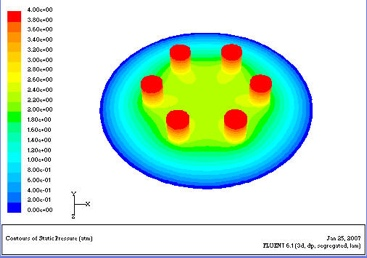
\includegraphics[height=2.5cm]{/pressure25.jpg}}
  \bicaption{包含子图题的范例(使用 subcaptionbox)}
            {Example with subcaptionbox}
  \label{fig:bisubcaptionbox}
\end{figure}

\pkg{subcaption} 宏包也提供了 \pkg{subfigure} 和 \pkg{subtable} 环境,如
图~\ref{fig:subfigure}。

\begin{figure}[!htp]
  \centering
  \begin{subfigure}{0.3\textwidth}
    \centering
    
\includegraphics[height=2cm]{./pdf/sjtu-badge.pdf}
    \caption{校徽}
  \end{subfigure}
  \hspace{1cm}
  \begin{subfigure}{0.4\textwidth}
    \centering
    
\includegraphics[height=1.5cm]{./pdf/sjtu-name.pdf}
    \caption{校名。注意这个图略矮些,subfigure 中同一行的子图在顶端对齐。}
  \end{subfigure}
  \caption{包含子图题的范例(使用 subfigure)}
  \label{fig:subfigure}
\end{figure}

Lorem ipsum dolor sit amet, consectetur adipisici elit, sed do eiusmod tempor
incididunt ut labore et dolore magna aliqua. Ut enim ad minim veniam, quis
nostrud exercitation ullamco laboris nisi ut aliquip ex ea commodo consequat.
Duis aute irure dolor in reprehenderit in voluptate velit esse cillum dolore eu
fugiat nulla pariatur. Excepteur sint occaecat cupidatat non proident, sunt in
culpa qui officia deserunt mollit anim id est laborum.

\section{表格}

\subsection{基本表格}

编排表格应简单明了,表达一致,明晰易懂,表文呼应、内容一致。表题置于表上,研究生
学位论文可以用中、英文两种文字居中排写,中文在上,也可以只用中文。

表格的编排建议采用国际通行的三线表\footnote{三线表,以其形式简洁、功能分明、阅读
方便而在科技论文中被推荐使用。三线表通常只有 3 条线,即顶线、底线和栏目线,没有
竖线。}。三线表可以使用 \pkg{booktabs} 提供的 \cs{toprule}、\cs{midrule} 和
\cs{bottomrule}。它们与 \pkg{longtable} 能很好的配合使用。

\begin{table}[!hpt]
  \caption[一个颇为标准的三线表]{一个颇为标准的三线表\footnotemark}
  \label{tab:firstone}
  \centering
  \begin{tabular}{@{}llr@{}} \toprule
    \multicolumn{2}{c}{Item} \\ \cmidrule(r){1-2}
    Animal & Description & Price (\$)\\ \midrule
    Gnat  & per gram  & 13.65 \\
          & each      & 0.01 \\
    Gnu   & stuffed   & 92.50 \\
    Emu   & stuffed   & 33.33 \\
    Armadillo & frozen & 8.99 \\ \bottomrule
  \end{tabular}
\end{table}
\footnotetext{这个例子来自
  \href{https://mirrors.sjtug.sjtu.edu.cn/ctan/macros/latex/contrib/booktabs/booktabs.pdf}%
  {《Publication quality tables in LaTeX》}(\pkg{booktabs} 宏包的文档)。这也是
  一个在表格中使用脚注的例子,请留意与 \pkg{threeparttable} 实现的效果有何不
  同。}

\subsection{复杂表格}

我们经常会在表格下方标注数据来源,或者对表格里面的条目进行解释。可以用
\pkg{threeparttable} 实现带有脚注的表格,如表~\ref{tab:footnote}。

\begin{table}[!htpb]
  \bicaption{一个带有脚注的表格的例子}{A Table with footnotes}
  \label{tab:footnote}
  \centering
  \begin{threeparttable}[b]
     \begin{tabular}{ccd{4}cccc}
      \toprule
      \multirow{2}*{total} & \multicolumn{2}{c}{20\tnote{a}} & \multicolumn{2}{c}{40} & \multicolumn{2}{c}{60} \\
      \cmidrule(lr){2-3}\cmidrule(lr){4-5}\cmidrule(lr){6-7}
      & www & \multicolumn{1}{c}{k} & www & k & www & k \\ % 使用说明符 d 的列会自动进入数学模式,使用 \multicolumn 对文字表头做特殊处理
      \midrule
      & $\underset{(2.12)}{4.22}$ & 120.0140\tnote{b} & 333.15 & 0.0411 & 444.99 & 0.1387 \\
      & 168.6123 & 10.86 & 255.37 & 0.0353 & 376.14 & 0.1058 \\
      & 6.761    & 0.007 & 235.37 & 0.0267 & 348.66 & 0.1010 \\
      \bottomrule
    \end{tabular}
    \begin{tablenotes}
    \item [a] the first note.% or \item [a]
    \item [b] the second note.% or \item [b]
    \end{tablenotes}
  \end{threeparttable}
\end{table}

Lorem ipsum dolor sit amet, consectetur adipisici elit, sed do eiusmod tempor
incididunt ut labore et dolore magna aliqua. Ut enim ad minim veniam, quis
nostrud exercitation ullamco laboris nisi ut aliquip ex ea commodo consequat.
Duis aute irure dolor in reprehenderit in voluptate velit esse cillum dolore eu
fugiat nulla pariatur. Excepteur sint occaecat cupidatat non proident, sunt in
culpa qui officia deserunt mollit anim id est laborum.

如某个表需要转页接排,可以用 \pkg{longtable} 实现。接排时表题省略,表头应重复书
写,并在右上方写“续表 xx”,如表~\ref{tab:performance}。

\begin{longtable}[c]{c*{6}{r}}
  \bicaption{实验数据}{Experimental data}
  \label{tab:performance} \\
  \toprule
  测试程序 & \multicolumn{1}{c}{正常运行} & \multicolumn{1}{c}{同步}
    & \multicolumn{1}{c}{检查点} & \multicolumn{1}{c}{卷回恢复}
    & \multicolumn{1}{c}{进程迁移} & \multicolumn{1}{c}{检查点} \\
   & \multicolumn{1}{c}{时间 (s)} & \multicolumn{1}{c}{时间 (s)}
    & \multicolumn{1}{c}{时间 (s)} & \multicolumn{1}{c}{时间 (s)}
    & \multicolumn{1}{c}{时间 (s)} &  文件(KB)\\
  \midrule
  \endfirsthead
  \multicolumn{7}{r}{续表~\thetable} \\
  \toprule
  测试程序 & \multicolumn{1}{c}{正常运行} & \multicolumn{1}{c}{同步}
    & \multicolumn{1}{c}{检查点} & \multicolumn{1}{c}{卷回恢复}
    & \multicolumn{1}{c}{进程迁移} & \multicolumn{1}{c}{检查点} \\
   & \multicolumn{1}{c}{时间 (s)} & \multicolumn{1}{c}{时间 (s)}
    & \multicolumn{1}{c}{时间 (s)} & \multicolumn{1}{c}{时间 (s)}
    & \multicolumn{1}{c}{时间 (s)}&  文件(KB)\\
  \midrule
  \endhead
  \hline
  \multicolumn{7}{r}{续下页}
  \endfoot
  \endlastfoot
  CG.A.2 & 23.05 & 0.002 & 0.116 & 0.035 & 0.589 & 32491 \\
  CG.A.4 & 15.06 & 0.003 & 0.067 & 0.021 & 0.351 & 18211 \\
  CG.A.8 & 13.38 & 0.004 & 0.072 & 0.023 & 0.210 & 9890 \\
  CG.B.2 & 867.45 & 0.002 & 0.864 & 0.232 & 3.256 & 228562 \\
  CG.B.4 & 501.61 & 0.003 & 0.438 & 0.136 & 2.075 & 123862 \\
  CG.B.8 & 384.65 & 0.004 & 0.457 & 0.108 & 1.235 & 63777 \\
  MG.A.2 & 112.27 & 0.002 & 0.846 & 0.237 & 3.930 & 236473 \\
  MG.A.4 & 59.84 & 0.003 & 0.442 & 0.128 & 2.070 & 123875 \\
  MG.A.8 & 31.38 & 0.003 & 0.476 & 0.114 & 1.041 & 60627 \\
  MG.B.2 & 526.28 & 0.002 & 0.821 & 0.238 & 4.176 & 236635 \\
  MG.B.4 & 280.11 & 0.003 & 0.432 & 0.130 & 1.706 & 123793 \\
  MG.B.8 & 148.29 & 0.003 & 0.442 & 0.116 & 0.893 & 60600 \\
  LU.A.2 & 2116.54 & 0.002 & 0.110 & 0.030 & 0.532 & 28754 \\
  LU.A.4 & 1102.50 & 0.002 & 0.069 & 0.017 & 0.255 & 14915 \\
  LU.A.8 & 574.47 & 0.003 & 0.067 & 0.016 & 0.192 & 8655 \\
  LU.B.2 & 9712.87 & 0.002 & 0.357 & 0.104 & 1.734 & 101975 \\
  LU.B.4 & 4757.80 & 0.003 & 0.190 & 0.056 & 0.808 & 53522 \\
  LU.B.8 & 2444.05 & 0.004 & 0.222 & 0.057 & 0.548 & 30134 \\
  EP.A.2 & 123.81 & 0.002 & 0.010 & 0.003 & 0.074 & 1834 \\
  EP.A.4 & 61.92 & 0.003 & 0.011 & 0.004 & 0.073 & 1743 \\
  EP.A.8 & 31.06 & 0.004 & 0.017 & 0.005 & 0.073 & 1661 \\
  EP.B.2 & 495.49 & 0.001 & 0.009 & 0.003 & 0.196 & 2011 \\
  EP.B.4 & 247.69 & 0.002 & 0.012 & 0.004 & 0.122 & 1663 \\
  EP.B.8 & 126.74 & 0.003 & 0.017 & 0.005 & 0.083 & 1656 \\
  SP.A.2 & 123.81 & 0.002 & 0.010 & 0.003 & 0.074 & 1854 \\
  SP.A.4 & 51.92 & 0.003 & 0.011 & 0.004 & 0.073 & 1543 \\
  SP.A.8 & 31.06 & 0.004 & 0.017 & 0.005 & 0.073 & 1671 \\
  SP.B.2 & 495.49 & 0.001 & 0.009 & 0.003 & 0.196 & 2411 \\
  SP.B.4 & 247.69 & 0.002 & 0.014 & 0.006 & 0.152 & 2653 \\
  SP.B.8 & 126.74 & 0.003 & 0.017 & 0.005 & 0.082 & 1755 \\
  \bottomrule
\end{longtable}

\section{算法环境}

算法环境可以使用 \pkg{algorithms} 宏包或者较新的 \pkg{algorithm2e} 实现。
算法~\ref{algo:algorithm} 是一个使用 \pkg{algorithm2e} 的例子。关于排版算法环境
的具体方法,请阅读相关宏包的官方文档。

\begin{algorithm}[htb]
  \caption{算法示例}
  \label{algo:algorithm}
  \small
  \SetAlgoLined
  \KwData{this text}
  \KwResult{how to write algorithm with \LaTeXe }

  initialization\;
  \While{not at end of this document}{
    read current\;
    \eIf{understand}{
      go to next section\;
      current section becomes this one\;
    }{
      go back to the beginning of current section\;
    }
  }
\end{algorithm}

\section{代码环境}

我们可以在论文中插入算法,但是不建议插入大段的代码。如果确实需要插入代码,建议使
用 \pkg{listings} 宏包。

\begin{codeblock}[language=C]
#include <stdio.h>
#include <unistd.h>
#include <sys/types.h>
#include <sys/wait.h>

int main() {
  pid_t pid;

  switch ((pid = fork())) {
  case -1:
    printf("fork failed\n");
    break;
  case 0:
    /* child calls exec */
    execl("/bin/ls", "ls", "-l", (char*)0);
    printf("execl failed\n");
    break;
  default:
    /* parent uses wait to suspend execution until child finishes */
    wait((int*)0);
    printf("is completed\n");
    break;
  }

  return 0;
}
\end{codeblock}

% !TEX root = ../thesis.tex

\chapter{数学与引用文献的标注}

\section{数学}

\subsection{数字和单位}

宏包 \pkg{siunitx} 提供了更好的数字和单位支持:
\begin{itemize}
  \item \num{12345.67890}
  \item \num{1+-2i}
  \item \num{.3e45}
  \item \num{1.654 x 2.34 x 3.430}
  \item \si{kg.m.s^{-1}}
  \item \si{\micro\meter} $\si{\micro\meter}$
  \item \si{\ohm} $\si{\ohm}$
  \item \numlist{10;20}
  \item \numlist{10;20;30}
  \item \SIlist{0.13;0.67;0.80}{\milli\metre}
  \item \numrange{10}{20}
  \item \SIrange{10}{20}{\degreeCelsius}
\end{itemize}

\subsection{数学符号和公式}

微分符号 $\dif$ 应使用正体,本模板提供了 \cs{dif} 命令。除此之外,模板还提供了一
些命令方便使用:
\begin{itemize}
  \item 圆周率 $\uppi$:\verb|\uppi|
  \item 自然对数的底 $\upe$:\verb|\upe|
  \item 虚数单位 $\upi$, $\upj$:\verb|\upi| \verb|\upj|
\end{itemize}

公式应另起一行居中排版。公式后应注明编号,按章顺序编排,编号右端对齐。
\begin{equation}
  \upe^{\upi\uppi} + 1 = 0,
\end{equation}
\begin{equation}
  \frac{\dif^2 u}{\dif t^2} = \int f(x) \dif x.
\end{equation}

公式末尾是需要添加标点符号的,至于用逗号还是句号,取决于公式下面一句是接着公式说的,还是另起一句。
\begin{equation}
		\frac{2h}{\pi}\int_{0}^{\infty}\frac{\sin\left( \omega\delta \right)}{\omega}
		\cos\left( \omega x \right) \dif\omega = 
		\begin{cases}
				h, \ \left| x \right| < \delta, \\
				\frac{h}{2}, \ x = \pm \delta, \\
				0, \ \left| x \right| > \delta.
		\end{cases}
\end{equation}
公式较长时最好在等号“$=$”处转行。
\begin{align}
    & I (X_3; X_4) - I (X_3; X_4 \mid X_1) - I (X_3; X_4 \mid X_2) \nonumber \\
  = & [I (X_3; X_4) - I (X_3; X_4 \mid X_1)] - I (X_3; X_4 \mid \tilde{X}_2) \\
  = & I (X_1; X_3; X_4) - I (X_3; X_4 \mid \tilde{X}_2).
\end{align}

如果在等号处转行难以实现,也可在 $+$、$-$、$\times$、$\div$运算符号处转行,转行
时运算符号仅书写于转行式前,不重复书写。
\begin{multline}
  \frac{1}{2} \Delta (f_{ij} f^{ij}) =
    2 \left(\sum_{i<j} \chi_{ij}(\sigma_{i} - \sigma_{j})^{2}
    + f^{ij} \nabla_{j} \nabla_{i} (\Delta f) \right. \\
  \left. + \nabla_{k} f_{ij} \nabla^{k} f^{ij} +
    f^{ij} f^{k} \left[2\nabla_{i}R_{jk}
    - \nabla_{k} R_{ij} \right] \vphantom{\sum_{i<j}} \right).
\end{multline}

\subsection{定理环境}

示例文件中使用 \pkg{ntheorem} 宏包配置了定理、引理和证明等环境。用户也可以使用
\pkg{amsthm} 宏包。

这里举一个“定理”和“证明”的例子。
\begin{theorem}[留数定理]
\label{thm:res}
  假设 $U$ 是复平面上的一个单连通开子集,$a_1, \ldots, a_n$ 是复平面上有限个点,
  $f$ 是定义在 $U \backslash \{a_1, \ldots, a_n\}$ 上的全纯函数,如果 $\gamma$
  是一条把 $a_1, \ldots, a_n$ 包围起来的可求长曲线,但不经过任何一个 $a_k$,并且
  其起点与终点重合,那么:

  \begin{equation}
    \label{eq:res}
    \ointop_\gamma f(z)\, \dif z = 2\uppi \upi \sum_{k=1}^n \operatorname{I}(\gamma, a_k) \operatorname{Res}(f, a_k).
  \end{equation}

  如果 $\gamma$ 是若尔当曲线,那么 $\operatorname{I}(\gamma, a_k) = 1$,因此:

  \begin{equation}
    \label{eq:resthm}
    \ointop_\gamma f(z)\, \dif z = 2\uppi \upi \sum_{k=1}^n \operatorname{Res}(f, a_k).
  \end{equation}

  在这里,$\operatorname{Res}(f, a_k)$ 表示 $f$ 在点 $a_k$ 的留数,
  $\operatorname{I}(\gamma, a_k)$ 表示 $\gamma$ 关于点 $a_k$ 的卷绕数。卷绕数是
  一个整数,它描述了曲线 $\gamma$ 绕过点 $a_k$ 的次数。如果 $\gamma$ 依逆时针方
  向绕着 $a_k$ 移动,卷绕数就是一个正数,如果 $\gamma$ 根本不绕过 $a_k$,卷绕数
  就是零。

  定理~\ref{thm:res} 的证明。

  \begin{proof}
    首先,由……

    其次,……

    所以……
  \end{proof}
\end{theorem}

\section{引用文献的标注}

按照教务处的要求,参考文献外观应符合国标 GB/T 7714 的要求。模版使用 \BibLaTeX\
配合 \pkg{biblatex-gb7714-2015} 样式包
\footnote{\url{https://www.ctan.org/pkg/biblatex-gb7714-2015}}
控制参考文献的输出样式,后端采用 \pkg{biber} 管理文献。

请注意 \pkg{biblatex-gb7714-2015} 宏包 2016 年 9 月才加入 CTAN,如果你使用的
\TeX\ 系统版本较旧,可能没有包含 \pkg{biblatex-gb7714-2015} 宏包,需要手动安装。
\BibLaTeX\ 与 \pkg{biblatex-gb7714-2015} 目前在活跃地更新,为避免一些兼容性问
题,推荐使用较新的版本。

正文中引用参考文献时,使用 \verb|\cite{key1,key2,key3...}| 可以产生“上标引用的
参考文献”,如 \cite{Meta_CN,chen2007act,DPMG}。使用
\verb|\parencite{key1,key2,key3...}| 则可以产生水平引用的参考文献,例如
\parencite{JohnD,zhubajie,IEEE-1363}。请看下面的例子,将会穿插使用水平的和上标的
参考文献:关于书的\parencite{Meta_CN,JohnD,IEEE-1363},关于期刊的
\cite{chen2007act,chen2007ewi},会议论文 \parencite{DPMG,kocher99,cnproceed},硕
士学位论文\parencite{zhubajie,metamori2004},博士学位论文
\cite{shaheshang,FistSystem01,bai2008},标准文件 \parencite{IEEE-1363},技术报告
\cite{NPB2},电子文献 \parencite{xiaoyu2001, CHRISTINE1998},用户手册
\parencite{RManual}。

当需要将参考文献条目加入到文献表中但又不在正文中引用,可以使用
\verb|\nocite{key1,key2,key3...}|。使用 \verb|\nocite{*}| 可以将参考文献数据库中
的所有条目加入到文献表中。

% !TEX root = ../thesis.tex

\begin{summary}
这里是全文总结内容。

2015 年 2 月 28 日,中央在北京召开全国精神文明建设工作表彰暨学雷锋志愿服务大会,
公布全国文明城市(区)、文明村镇、文明单位名单。上海交通大学荣获全国文明单位称
号。

全国文明单位这一荣誉是对交大人始终高度重视文明文化工作的肯定,是对交大长期以来文
明创建工作成绩的褒奖。在学校党委、文明委的领导下,交大坚持将文明创建工作纳入学校
建设世界一流大学的工作中,全体师生医护员工群策群力、积极开拓,落实国家和上海市有
关文明创建的各项要求,以改革创新、科学发展为主线,以质量提升为目标,聚焦文明创建
工作出现的重点和难点,优化文明创建工作机制,传播学校良好形象,提升社会美誉度,显
著增强学校软实力。2007 至 2012 年间,上海交大连续三届荣获“上海市文明单位”称
号,成为创建全国文明单位的新起点。

上海交大自启动争创全国文明单位工作以来,凝魂聚气、改革创新,积极培育和践行社会主
义核心价值观。坚持统筹兼顾、多措并举,将争创全国文明单位与学校各项中心工作紧密结
合,着力构建学校文明创建新格局,不断提升师生医护员工文明素养,以“冲击世界一流大
学汇聚强大精神动力”为指导思想,以“聚焦改革、多元推进、以评促建、丰富内涵、彰显
特色”为工作原则,并由全体校领导群策领衔“党的建设深化、思想教育深入、办学成绩显
著、大学文化丰富、校园环境优化、社会责任担当”六大板块共 28 项重点突破工作,全面
展现近年来交大文明创建工作的全貌和成就。

进入新阶段,学校将继续开拓文明创建工作新格局,不断深化工作理念和工作实践,创新工
作载体、丰富活动内涵、凸显创建成效,积极服务于学校各项中心工作和改革发展的大局
面,在上级党委、文明委的关心下,在学校党委的直接领导下,与时俱进、开拓创新,为深
化内涵建设、加快建成世界一流大学、推动国家进步和社会发展而努力奋斗!

上海交通大学医学院附属仁济医院也获得全国文明单位称号。
\end{summary}


% 使用英文字母对附录编号
\appendix

% 附录内容,本科学位论文可以用翻译的文献替代。
% !TEX root = ../thesis.tex

\chapter{Maxwell Equations}

选择二维情况,有如下的偏振矢量:
\begin{subequations}
  \begin{align}
    {\bf E} &= E_z(r, \theta) \hat{\bf z}, \\
    {\bf H} &= H_r(r, \theta) \hat{\bf r} + H_\theta(r, \theta) \hat{\bm\theta}.
  \end{align}
\end{subequations}
对上式求旋度:
\begin{subequations}
  \begin{align}
    \nabla \times {\bf E} &= \frac{1}{r} \frac{\partial E_z}{\partial\theta}
      \hat{\bf r} - \frac{\partial E_z}{\partial r} \hat{\bm\theta}, \\
    \nabla \times {\bf H} &= \left[\frac{1}{r} \frac{\partial}{\partial r}
      (r H_\theta) - \frac{1}{r} \frac{\partial H_r}{\partial\theta} \right]
      \hat{\bf z}.
  \end{align}
\end{subequations}
因为在柱坐标系下,$\overline{\overline\mu}$ 是对角的,所以 Maxwell 方程组中电场
$\bf E$ 的旋度:
\begin{subequations}
  \begin{align}
    & \nabla \times {\bf E} = \upi \omega {\bf B}, \\
    & \frac{1}{r} \frac{\partial E_z}{\partial\theta} \hat{\bf r} -
      \frac{\partial E_z}{\partial r}\hat{\bm\theta} = \upi \omega \mu_r H_r
      \hat{\bf r} + \upi \omega \mu_\theta H_\theta \hat{\bm\theta}.
  \end{align}
\end{subequations}
所以 $\bf H$ 的各个分量可以写为:
\begin{subequations}
  \begin{align}
    H_r &= \frac{1}{\upi \omega \mu_r} \frac{1}{r}
      \frac{\partial E_z}{\partial\theta}, \\
    H_\theta &= -\frac{1}{\upi \omega \mu_\theta}
      \frac{\partial E_z}{\partial r}.
  \end{align}
\end{subequations}
同样地,在柱坐标系下,$\overline{\overline\epsilon}$ 是对角的,所以 Maxwell 方程
组中磁场 $\bf H$ 的旋度:
\begin{subequations}
  \begin{align}
    & \nabla \times {\bf H} = -\upi \omega {\bf D}, \\
    & \left[\frac{1}{r} \frac{\partial}{\partial r}(r H_\theta) - \frac{1}{r}
      \frac{\partial H_r}{\partial\theta} \right] \hat{\bf z} = -\upi \omega
      {\overline{\overline\epsilon}} {\bf E} = -\upi \omega \epsilon_z E_z
      \hat{\bf z}, \\
    & \frac{1}{r} \frac{\partial}{\partial r}(r H_\theta) - \frac{1}{r}
      \frac{\partial H_r}{\partial\theta} = -\upi \omega \epsilon_z E_z.
  \end{align}
\end{subequations}
由此我们可以得到关于 $E_z$ 的波函数方程:
\begin{equation}
  \frac{1}{\mu_\theta \epsilon_z} \frac{1}{r} \frac{\partial}{\partial r}
  \left(r \frac{\partial E_z}{\partial r} \right) + \frac{1}{\mu_r \epsilon_z}
  \frac{1}{r^2} \frac{\partial^2E_z}{\partial\theta^2} +\omega^2 E_z = 0.
\end{equation}

% !TEX root = ../thesis.tex

\chapter{绘制流程图}

图~\ref{fig:flow_chart} 是一张流程图示意。使用 \pkg{tikz} 环境,搭配四种预定义节
点(\verb+startstop+、\verb+process+、\verb+decision+和\verb+io+),可以容易地绘
制出流程图。

\begin{figure}[!htp]
  \centering
  \resizebox{6cm}{!}{\begin{tikzpicture}[node distance=2cm]
    \node (pic) [startstop] {待测图片};
    \node (bg) [io, below of=pic] {读取背景};
    \node (pair) [process, below of=bg] {匹配特征点对};
    \node (threshold) [decision, below of=pair, yshift=-0.5cm] {多于阈值};
    \node (clear) [decision, right of=threshold, xshift=3cm] {清晰?};
    \node (capture) [process, right of=pair, xshift=3cm, yshift=0.5cm] {重采};
    \node (matrix_p) [process, below of=threshold, yshift=-0.8cm] {透视变换矩阵};
    \node (matrix_a) [process, right of=matrix_p, xshift=3cm] {仿射变换矩阵};
    \node (reg) [process, below of=matrix_p] {图像修正};
    \node (return) [startstop, below of=reg] {配准结果};
     
    %连接具体形状
    \draw [arrow](pic) -- (bg);
    \draw [arrow](bg) -- (pair);
    \draw [arrow](pair) -- (threshold);

    \draw [arrow](threshold) -- node[anchor=south] {否} (clear);

    \draw [arrow](clear) -- node[anchor=west] {否} (capture);
    \draw [arrow](capture) |- (pic);
    \draw [arrow](clear) -- node[anchor=west] {是} (matrix_a);
    \draw [arrow](matrix_a) |- (reg);

    \draw [arrow](threshold) -- node[anchor=east] {是} (matrix_p);
    \draw [arrow](matrix_p) -- (reg);
    \draw [arrow](reg) -- (return);
\end{tikzpicture}
}
  \bicaption{绘制流程图效果}{Flow chart}
  \label{fig:flow_chart}
\end{figure}


% 文后无编号部分
\backmatter

% 参考资料
\printbibliography[heading=bibintoc]

% 用于盲审的论文需隐去致谢、发表论文、参与项目、申请专利、简历

% 致谢
% !TEX root = ../thesis.tex

%TC:ignore

\begin{acknowledgements}
  感谢那位最先制作出博士学位论文 \LaTeX 模板的交大物理系同学!

  感谢 William Wang 同学对模板移植做出的巨大贡献!

  感谢 \href{https://github.com/weijianwen}{@weijianwen} 学长一直以来的开发和维
  护工作!

  感谢 \href{https://github.com/sjtug}{@sjtug} 以及
   \href{https://github.com/dyweb}{@dyweb} 对 0.9.5 之后版本的开发和维护工作!

  感谢所有为模板贡献过代码的同学们, 以及所有测试和使用模板的各位同学!

  感谢 \LaTeX 和 \href{https://github.com/sjtug/SJTUThesis}{\sjtuthesis},帮我节
  省了不少时间。
\end{acknowledgements}

%TC:endignore


% 发表论文、参与项目、申请专利、简历
% 盲审论文中,发表学术论文及参与科研情况等仅以第几作者注明即可,不要出现作者或他人姓名
% % !TEX root = ../thesis.tex

%TC:ignore

\begin{publications}
  \item Chen H, Chan C~T. Acoustic cloaking in three dimensions using acoustic metamaterials[J]. Applied Physics Letters, 2007, 91:183518.
  \item Chen H, Wu B~I, Zhang B, et al. Electromagnetic Wave Interactions with a Metamaterial Cloak[J]. Physical Review Letters, 2007, 99(6):63903.
\end{publications}

\begin{publications*}
  \item 第一作者. 中文核心期刊论文, 2007.
  \item 第一作者. EI 国际会议论文, 2006.
\end{publications*}

%TC:endignore

% % !TEX root = ../thesis.tex

%TC:ignore

\begin{projects}
  \item 参与973项目子课题(2007年6月--2008年5月)
  \item 参与自然基金项目(2005年5月--2005年8月)
  \item 参与国防项目(2005年8月--2005年10月)
\end{projects}

\begin{projects*}
  \item 973项目“XXX”
  \item 自然基金项目“XXX”
  \item 国防项目“XXX”
\end{projects*}

%TC:endignore

% % !TEX root = ../thesis.tex

%TC:ignore

\begin{patents}
  \item 第一发明人,“永动机”,专利申请号202510149890.0
\end{patents}

\begin{patents*}
  \item 第一发明人,“永动机”,专利申请号XXXXXXXXXXXX.X
\end{patents*}

%TC:endignore

% % !TEX root = ../thesis.tex

%TC:ignore

\begin{resume}
  \subsection*{基本情况}
    某某,yyyy 年 mm 月生于 xxxx。

  \subsection*{教育背景}
  \begin{itemize}
    \item yyyy 年 mm 月至今,上海交通大学,博士研究生,xx 专业
    \item yyyy 年 mm 月至 yyyy 年 mm 月,上海交通大学,硕士研究生,xx 专业
    \item yyyy 年 mm 月至 yyyy 年 mm 月,上海交通大学,本科,xx 专业
  \end{itemize}

  \subsection*{研究兴趣}
    \LaTeX{} 排版

  \subsection*{联系方式}
  \begin{itemize}
    \item 地址: 上海市闵行区东川路 800 号,200240
    \item E-mail: \email{xxx@sjtu.edu.cn}
  \end{itemize}
\end{resume}

%TC:endignore


% 中文学士学位论文要求在最后有一个英文大摘要,单独编页码,英文学士学位论文不需要
% !TEX root = ../thesis.tex

\begin{bigabstract}
  An imperial edict issued in 1896 by Emperor Guangxu, established Nanyang
  Public School in Shanghai. The normal school, school of foreign studies,
  middle school and a high school were established. Sheng Xuanhuai, the person
  responsible for proposing the idea to the emperor, became the first president
  and is regarded as the founder of the university.

  During the 1930s, the university gained a reputation of nurturing top
  engineers. After the foundation of People's Republic, some faculties were
  transferred to other universities. A significant amount of its faculty were
  sent in 1956, by the national government, to Xi'an to help build up Xi'an Jiao
  Tong University in western China. Afterwards, the school was officially
  renamed Shanghai Jiao Tong University.

  Since the reform and opening up policy in China, SJTU has taken the lead in
  management reform of institutions for higher education, regaining its vigor
  and vitality with an unprecedented momentum of growth. SJTU includes five
  beautiful campuses, Xuhui, Minhang, Luwan Qibao, and Fahua, taking up an area
  of about 3,225,833 m2. A number of disciplines have been advancing towards the
  top echelon internationally, and a batch of burgeoning branches of learning
  have taken an important position domestically.

  Today SJTU has 31 schools (departments), 63 undergraduate programs, 250
  masters-degree programs, 203 Ph.D. programs, 28 post-doctorate programs, and
  11 state key laboratories and national engineering research centers.

  SJTU boasts a large number of famous scientists and professors, including 35
  academics of the Academy of Sciences and Academy of Engineering, 95 accredited
  professors and chair professors of the "Cheung Kong Scholars Program" and more
  than 2,000 professors and associate professors.

  Its total enrollment of students amounts to 35,929, of which 1,564 are
  international students. There are 16,802 undergraduates, and 17,563 masters
  and Ph.D. candidates. After more than a century of operation, Jiao Tong
  University has inherited the old tradition of "high starting points, solid
  foundation, strict requirements and extensive practice." Students from SJTU
  have won top prizes in various competitions, including ACM International
  Collegiate Programming Contest, International Mathematical Contest in Modeling
  and Electronics Design Contests. Famous alumni include Jiang Zemin, Lu Dingyi,
  Ding Guangen, Wang Daohan, Qian Xuesen, Wu Wenjun, Zou Taofen, Mao Yisheng,
  Cai Er, Huang Yanpei, Shao Lizi, Wang An and many more. More than 200 of the
  academics of the Chinese Academy of Sciences and Chinese Academy of
  Engineering are alumni of Jiao Tong University.
\end{bigabstract}


\end{document}
